%% For normal draft builds (figs undisplayed hence fast compile)
%\documentclass[hyperpdf,nobind,draft,oneside]{hepthesis}
%\documentclass[hyperpdf,nobind,draft,twoside]{hepthesis}

%% For short draft builds (breaks citations by necessity)
%\documentclass[hyperpdf,nobind,draft,hidefrontback]{hepthesis}

%% For Cambridge soft-bound version
\documentclass[hyperpdf,bindnopdf]{hepthesis}
%% For Cambridge hard-bound version (must be one-sided)
%\documentclass[hyperpdf,oneside]{hepthesis}

%% Load special font packages here if you wish
%\usepackage{lmodern}
%\usepackage{euler}

%% Put package includes etc. into preamble.tex for convenience
\usepackage{xspace}
\usepackage{tikz}
\usepackage{morefloats,afterpage}
\usepackage{mathrsfs} % script font
\usepackage{verbatim}
\usepackage{caption}
\usepackage{subcaption}
\usepackage{amsmath}
\usepackage{mathpazo}
\usepackage{rotating}
\usepackage{tabularx}

\usepackage{braket}

%% Using Babel allows other languages to be used and mixed-in easily
%\usepackage[ngerman,english]{babel}
\usepackage[english]{babel}
\selectlanguage{english}

\usepackage{epigraph}

%% Citation system tweaks
\usepackage{cite}
% \let\@OldCite\cite
% \renewcommand{\cite}[1]{\mbox{\!\!\!\@OldCite{#1}}}

%% Maths
\usepackage{abmath}
\DeclareRobustCommand{\mymath}[1]{\ensuremath{\maybebmsf{#1}}}
% \DeclareRobustCommand{\parenths}[1]{\mymath{\left({#1}\right)}\xspace}
% \DeclareRobustCommand{\braces}[1]{\mymath{\left\{{#1}\right\}}\xspace}
% \DeclareRobustCommand{\angles}[1]{\mymath{\left\langle{#1}\right\rangle}\xspace}
% \DeclareRobustCommand{\sqbracs}[1]{\mymath{\left[{#1}\right]}\xspace}
% \DeclareRobustCommand{\mods}[1]{\mymath{\left\lvert{#1}\right\rvert}\xspace}
% \DeclareRobustCommand{\modsq}[1]{\mymath{\mods{#1}^2}\xspace}
% \DeclareRobustCommand{\dblmods}[1]{\mymath{\left\lVert{#1}\right\rVert}\xspace}
% \DeclareRobustCommand{\expOf}[1]{\mymath{\exp{\!\parenths{#1}}}\xspace}
% \DeclareRobustCommand{\eexp}[1]{\mymath{e^{#1}}\xspace}
% \DeclareRobustCommand{\plusquad}{\mymath{\oplus}\xspace}
% \DeclareRobustCommand{\logOf}[1]{\mymath{\log\!\parenths{#1}}\xspace}
% \DeclareRobustCommand{\lnOf}[1]{\mymath{\ln\!\parenths{#1}}\xspace}
% \DeclareRobustCommand{\ofOrder}[1]{\mymath{\mathcal{O}\parenths{#1}}\xspace}
% \DeclareRobustCommand{\SOgroup}[1]{\mymath{\mathup{SO}\parenths{#1}}\xspace}
% \DeclareRobustCommand{\SUgroup}[1]{\mymath{\mathup{SU}\parenths{#1}}\xspace}
% \DeclareRobustCommand{\Ugroup}[1]{\mymath{\mathup{U}\parenths{#1}}\xspace}
% \DeclareRobustCommand{\I}[1]{\mymath{\mathrm{i}}\xspace}
% \DeclareRobustCommand{\colvector}[1]{\mymath{\begin{pmatrix}#1\end{pmatrix}}\xspace}
\DeclareRobustCommand{\Rate}{\mymath{\Gamma}\xspace}
\DeclareRobustCommand{\RateOf}[1]{\mymath{\Gamma}\parenths{#1}\xspace}


\newcolumntype{Y}{>{\centering\arraybackslash}X}
% T2K specific
\newcommand{\nue}{$\nu_{e}$}
\newcommand{\nueb}{$\bar{\nu}_{e}$}
\newcommand{\numu}{$\nu_{\mu}$}
\newcommand{\numub}{$\bar{\nu}_{\mu}$}
\newcommand{\nutau}{$\nu_{\tau}$}
\newcommand{\nuebar}{$\bar{\nu}_{e}$}
\newcommand{\numubar}{$\bar{\nu}_{\mu}$}

\newcommand{\sk}{SK}
\newcommand{\nd}{ND280}

\newcommand\red[1]{{\textit{\Large{\textbf{\color{red}#1}}}}}
\newcommand\blue[1]{{\textit{\Large{\textbf{\color{blue}#1}}}}}

\newcommand{\FGDCCNoPi}[2]{FGD{#1} CC$0\pi$ {#2}}
\newcommand{\FGDCCOnePi}[2]{FGD{#1} CC$1\pi$ {#2}}
\newcommand{\FGDCCOther}[2]{FGD{#1} CCOther {#2}}
\newcommand{\FGDCCOneTrk}[2]{FGD{#1} CC1Track {#2}}
\newcommand{\FGDCCNTrk}[2]{FGD{#1} CCNTrack {#2}}
\newcommand{\FGDCCnuOneTrk}[2]{FGD{#1} CC1Trk {#2}}
\newcommand{\FGDCCnuNTrk}[2]{FGD{#1} CCNTrk {#2}}
\newcommand{\pmu}{$p_\mu$}
\newcommand{\cosmu}{$\cos\theta_\mu$}

%% High-energy physics stuff
\usepackage{abhep}
\usepackage{hepnames}
\usepackage{hepunits}
\DeclareRobustCommand{\arXivCode}[1]{arXiv:#1}
\DeclareRobustCommand{\CP}{\ensuremath{\mathcal{CP}}\xspace}
\DeclareRobustCommand{\CPviolation}{\CP-violation\xspace}
\DeclareRobustCommand{\CPv}{\CPviolation}
\DeclareRobustCommand{\bphysics}{\Pbottom-physics\xspace}
\DeclareRobustCommand{\bhadron}{\Pbottom-hadron\xspace}
\DeclareRobustCommand{\Bmeson}{\PB-meson\xspace}
\DeclareRobustCommand{\bbaryon}{\Pbottom-baryon\xspace}
\DeclareRobustCommand{\Bdecay}{\PB-decay\xspace}
\DeclareRobustCommand{\bdecay}{\Pbottom-decay\xspace}
\DeclareRobustCommand{\BToKPi}{\HepProcess{ \PB \to \PK \Ppi }\xspace}
\DeclareRobustCommand{\BToPiPi}{\HepProcess{ \PB \to \Ppi \Ppi }\xspace}
\DeclareRobustCommand{\BToKK}{\HepProcess{ \PB \to \PK \PK }\xspace}
\DeclareRobustCommand{\BToRhoPi}{\HepProcess{ \PB \to \Prho \Ppi }\xspace}
\DeclareRobustCommand{\BToRhoRho}{\HepProcess{ \PB \to \Prho \Prho }\xspace}
\DeclareRobustCommand{\X}{\thesismath{X}\xspace}
\DeclareRobustCommand{\Xbar}{\thesismath{\overline{X}}\xspace}
\DeclareRobustCommand{\Xzero}{\HepGenParticle{X}{}{0}\xspace}
\DeclareRobustCommand{\Xzerobar}{\HepGenAntiParticle{X}{}{0}\xspace}
\DeclareRobustCommand{\epluseminus}{\Ppositron\!\Pelectron\xspace}
\DeclareRobustCommand{\protonproton}{\Pproton\APantiproton\xspace}


%% You can set the line spacing this way
%\setallspacing{double}
%% or a section at a time like this
%\setfrontmatterspacing{double}


%% Define the thesis title and author
\title{Minimising systematic uncertainties in the T2K experiment by use of near-detector and external data}
\author{Clarence Wret}

%% Doc-specific PDF metadata
\makeatletter
\@ifpackageloaded{hyperref}{
\hypersetup{
  pdftitle = {Minimising systematic uncertainties in the T2K experiment by use of near-detector and external data},
  pdfsubject = {Clarence Wret, PhD thesis},
  pdfkeywords = {T2K, neutrino physics, neutrino oscillations},
  pdfauthor = {\textcopyright\ Clarence Wret}
}}{}
\makeatother


%% Start the document
\begin{document}

%% Define the un-numbered front matter (cover pages, rubrik and table of contents)
\begin{frontmatter}
  %% Title
\titlepage[The Blackett Laboratory,\\Imperial College London]{A Dissertation Submitted to Imperial College London\\ for the Degree of Doctor of Philosophy}

%% Abstract
\begin{abstract}[\LARGE{\textbf{\thetitle}}\\ \vspace*{1.5cm} \normalsize{\textit{Abstract}}]
	The Tokai to Kamioka (T2K) long baseline neutrino oscillation experiment was designed to make precise measurements of neutrino oscillations. It uses a muon (anti-)neutrino dominated beam produced at the Japan Proton Accelerator Research Complex (J-PARC) on the east coast of Japan, aiming towards the Super-Kamiokande (SK) detector 295 km west. The neutrino beam is sampled by the two near detectors ND280 and INGRID, 280 m downstream of production. These measure the neutrino flux and interaction cross-sections to reduce the impact of systematics for oscillation analyses. The work presented herein details the process of using ND280, INGRID, and external data to best constrain the predicted event rates at SK. The analysis proceeds by using a Markov Chain Monte Carlo method which simultaneously fits ND280 and SK data without assumptions on the underlying posterior probability density function. The two analyses detailed here reduce event rate uncertainties at SK from 12-14\% to 2-4\%, enabling world-leading oscillation parameters to be extracted from T2K. Numerous run-by-run and detector-by-detector studies were performed and alternate models investigated, all of which were deemed compatible within error. The work has been included in the official T2K results presented in 2017 and 2018, and its use continues beyond that.
\end{abstract}

%% Declaration
\begin{declaration}
  This dissertation is the result of my own work, except where explicit reference is made to the work of others, and has not been submitted for another qualification to this or any other university. This dissertation does not exceed the word limit for the respective Degree Committee.
  \vspace*{1cm}
  \begin{flushright}
	  \theauthor
  \end{flushright}
\end{declaration}

%% Acknowledgements
\begin{acknowledgements}
	I have had the great privilege to work, travel, and form friendships with a multitude of excellent people during my three years on T2K and at Imperial College London. Special mentions to all of those who have discussed lovely complex ideas at length with me on never-ending flights, speeding Shinkansens, in coffee shops, and on paradisal islands.
	
	Starting my Ph.D. on neutrino interactions and model selections, I am indebted to Patrick Stowell, Callum Wilkinson, Luke Pickering and Ryan Terri for countless hours of discussions and explanations, culminating in the birth of the NUISANCE project\cite{NUISANCE}---now in use across many neutrino interaction experiments. We could not have done it without the expertise and advice of my supervisor Morgan Wascko, Kendall Mahn, and Kevin McFarland. I also extend special gratitude to Minoo Kabirnezhad for our two months in Japan, implementing new single pion production models and eating noodles.
  
	Continuing the interaction model studies with ND280 data---the topic of this thesis---would have been impossible without the help of the current and past members of the MaCh3 analysis group, spearheaded by Asher Kaboth. I especially hail Asher for his many wisdoms on the fit mechanics, statistics and Markov Chain Monte Carlo and Richard Calland for fuelling my interest in multi-threading and GPU programming. I thank the members of the frequentist ND280 fitting group (BANFF), led by Mark Scott with Simon Bienstock and Pierre Lasorak, for many discussions and hard work on studying the physics, statistics and systematics in the fit.
	
	I remain grateful for the time spent and the knowledge transferred through my colleagues in the Imperial T2K group: you all made room 530 (and beyond) a treat and joy. I thank my classmates in the Imperial HEP group Jack Wright, Sioni Summers, Thibaud Humair, and Slavomira Stefkova for not always discussing physics at work, and making Imperial a very welcoming place to work.
	
	A modern High Energy Physics analysis demands excellent computing. The work in this thesis could not happen without the Compute Canada Guillimin, Cedar and Graham clusters---made possible by Hiro Tanaka---Imperial College High Energy Physics Computing---maintained by Simon Fayer and Ray Beuselinck, with special thanks to David Colling for GPU support---and the Imperial College High Performace Computing centre. I acknowledge the generous hardware sponsorship from NVIDIA's academic seeding project.
	
	Finally, I extend my deepest gratitude to my close friends and loved ones, my sister, parents, step-parent, and grandmother. Thank you for all the entertaining distractions, buckets of patience, endless support, and much love. I hope you forever remain in my life.
\end{acknowledgements}

%% ToC
\tableofcontents
\end{frontmatter}

%% Start the content body of the thesis
\begin{mainmatter}
  %% Actually, more semantic chapter filenames are better, like "chap-bgtheory.tex"
  \chapter{Neutrino Physics}
\label{chap:theory}
This chapter introduces the experimental evidence for the neutrino and neutrino oscillations, outlines the theory of neutrino oscillations, and discusses neutrino interactions in the $E_\nu\sim1-10 \text{ GeV}$ range, relevant to long baseline neutrino oscillation experiments.

\section{The Discoveries of the Neutrinos}
Neutrinos were initially proposed as a solution to the apparent violation of the conservation of four- and angular momentum in James Chadwick's measurements of beta decay in 1932\cite{Chadwick1,Chadwick2}. Inspired by Wolfgang Pauli's new elementary particle ``the neutron''\footnote{Which had characteristics of what we today call a nucleon and a neutrino}\cite{pauli_1933}, Enrico Fermi built his theory of $\beta$-decay\cite{fermi_1934}, in which the observable process $n \rightarrow p + e^-$ is always accompanied by an invisible four-momentum carrier, the electron anti-neutrino.

The neutrino remained elusive until Reines and Cowan in 1953 devised their experiments using the inverse beta decay (IBD) process, $\bar{\nu}_e + p \rightarrow n + e^+$, near a nuclear reactor\cite{reines_cowan_1,reines_cowan_2}. The experiment consisted of two tanks of water sandwiched by three liquid scintillator tanks with photo multiplier tubes (PMTs). The water was doped with 40 kg $\text{CdCl}_2$, which could detect free neutrons through capture. The electron anti-neutrinos were emitted by the nuclear reactor, interacted with the protons in the water, producing a prompt signal from $e^+ + e^- \rightarrow 2\gamma$. The free neutron was detected $\sim5\mu\text{s}$ after the prompt $2\gamma$ from $n + ^{108}\text{Cd} \rightarrow ^{109m}\text{Cd} \rightarrow ^{109}\text{Cd} + \gamma$. The experiment also took data from a reactor off period, demonstrating a significant reduction in neutrino event rates. Modern reactor neutrino oscillation experiments such as Daya Bay\cite{daya_bay} operate much on the same principle. The experiment was complemented by measurements by R. Davis  in 1964\cite{davis}, which exposed tanks of $^{37}\text{Cl}$ to reactor electron anti-neutrinos, interacting through $\bar{\nu}_e + ^{37}\text{Cl} \rightarrow e^- + ^{37}\text{Ar}$, which would violate lepton number conservation. The experiment found no excess of $^{37}\text{Ar}$, and instead set limits on the solar neutrino flux. 

The field quickly developed after the first measurements and in 1962 Lederman, Schwartz, Steinberger and others\cite{lederman} observed another flavour of neutrino, the muon neutrino. They used a beam of protons impinging a target, creating a $\pi$ dominated beam which decayed following $\pi^+ \rightarrow \mu^+ + \nu_\mu$, and looked for subsequent interactions of the $\nu_\mu$ in a 10 tonne shielded aluminium spark chamber. The experiment was later confirmed by measurements at CERN in 1964\cite{cern_spark,cern_spark2}.

When the third charged lepton, the $\tau$, was discovered at SLAC's $e^+e^-$ accelerator in 1975\cite{tau_disc}, the search for its neutrino partner started. Its existence was already hinted at in $\tau$ decays and was discovered at DONUT in 2000\cite{tau_nu_disc}. The discovery of the $\nu_\tau$ and the three neutrino flavours was largely expected from precise measurements of $Z$ decays at the Large Electron Positron (LEP) and the Stanford Linear Accelerator (SLAC), which found the number of active neutrino flavours, assuming the Standard Model, as $N_\nu = 2.9840\pm0.0082$\cite{lep}. This has also been confirmed by cosmological data from Planck and others, $N_\text{eff} = 3.04\pm0.18$\footnote{$N_\text{eff}=3.0\pm0.4$ and $\sum m_\nu < 0.22 \text{ eV}$ when varying both $N_\text{eff}$ and $\sum m_\nu$.}\cite{planck}.

\section{Neutrino Oscillations}
\label{sec:theory:osc}
The discovery of neutrino oscillations, detailed in \autoref{sec:exp_overview}, is a direct consequence of neutrino mass. B. Pontecorvo\cite{p1,p2,pontecorvo_gribov}, Z. Maki, M. Nakagawa and S. Sakata\cite{mns} developed the PMNS formalism, widely used by the oscillation community today. This section highlights some crucial components of the theory and how it has been applied in the field.

The PMNS formalism starts by introducing a neutrino mass eigenstate $\ket{\nu_i}$, which is a linear superposition of the flavour eigenstates participating in the weak interaction $\ket{\nu_\alpha}$ with $n$ neutrino states,
\begin{equation}
\ket{\nu_i} = \sum_\alpha^n U_{\alpha i} \ket{\nu_\alpha}
\end{equation}
where the unitary matrix $U$ is generally expressed as
\begin{equation}
U = 
\begin{pmatrix}
	U_{e 1} & U_{e 2} & U_{e 3} \\
	U_{\mu 1} & U_{\mu 2} & U_{\mu 3} \\
	U_{\tau 1} & U_{\tau 2} & U_{\tau 3} \\
\end{pmatrix}
\end{equation}
This echoes that of quark mixing proposed by Cabbibo\cite{cabbibo}, Kobayashi and Maskawa\cite{km}. The superposition leads to a probability of observing neutrino flavour change from flavour $\alpha$ to $\beta$ over distance $L$ for a neutrino with energy $E$ in which the square of two neutrino mass states are separated by $\Delta m_{ij}^2 = m^2_i - m^2_j$,
\begin{equation}
P(\nu_\alpha \rightarrow \nu_\beta) = |\braket{\nu_\beta|\nu_\alpha(t)}|^2 = \sum_{k,j} U^*_{\alpha k} U_{\beta k} U^*_{\alpha j} U_{\beta j} \exp{ \left( -i\frac{\Delta m^2_{i j} L}{2E} \right)}
\end{equation}
Then using the squared unitarity relation we finally get\cite{boris_mixing},
\begin{align}
P(\nu_\alpha \rightarrow \nu_\beta) = \delta_{\alpha \beta} &- 4\sum_{i>j} Re\left(U^*_{\alpha i} U_{\beta i} U_{\alpha j} U^*_{\beta j}\right)  \sin^2 ( \Delta m^2_{ij}\frac{L}{4E} ) \\
									&+(-) 2\sum_{i>j} Im\left( U^*_{\alpha i} U_{\beta i} U_{\alpha j} U^*_{\beta j} \right) \sin ( \Delta m^2_{ij}\frac{L}{2E} )
\end{align}
where the negative sign is picked up for anti-neutrinos.

The PMNS matrix is often parameterised into three separate matrices with their own mixing angles $\theta_{13},\theta_{23}$ and $\theta_{12}$ and a complex phase $\delta$, where $c_{ij}=\cos\theta_{ij}$ and $s_{ij}=\sin\theta_{ij}$\cite{boris_mixing},
\begin{equation}
U = 
\begin{pmatrix}
1 & 0 & 0 \\
0 & c_{23} & s_{23} \\
0 & -s_{23} & c_{23} \\
\end{pmatrix}
\begin{pmatrix}
c_{13} & 0 & s_{13}e^{-i\delta} \\
0 & 1 & 0 \\
-s_{13}e^{-i\delta} & 0 & c_{13} \\
\end{pmatrix}
\begin{pmatrix}
c_{12} & s_{12} & 0 \\
-s_{12} & c_{12} & 0 \\
0 & 0 & 1 \\
\end{pmatrix}
\end{equation}
where the $(1,2)$ parameters are referred to as ``solar'', $(2,3)$ as ``atmospheric'', and $(1,3)$ as ``reactor''. The $\delta$ is commonly referred to as the CP violating Dirac phase, $\delta_{CP}$. 

Reducing down to two neutrino mass states (where the third mass state is approximately degenerate with another mass state), we obtain a simpler mixing matrix $U$,
\begin{equation}
U = 
\begin{pmatrix}
\cos\theta & \sin\theta \\
- \sin\theta & \cos \theta \\
\end{pmatrix}
\end{equation}
and an oscillation probability of
\begin{equation}
P(\nu_\alpha \rightarrow \nu_\beta) = \delta_{\alpha \beta} -(+) \sin^2 \left( 2\theta \right) \sin^2 \left( \frac{1.267 \Delta m^2 \left[\text{eV}^2\right] L\left[\text{km}\right]}{E\left[\text{GeV}\right]} \right)
\label{eq:two_flavour}
\end{equation}
where the positive sign is picked up when $\beta \neq \alpha$. The sinusoidal oscillation of the neutrino flavour states in \autoref{eq:two_flavour} has a period controlled by the parameter $\Delta m^2$ and amplitude by the mixing angle $\theta$. The maximum oscillation probability for a fixed mixing angle $\theta$ is at $L/E \sim 1.25/\Delta m^2$, which for $\Delta m^2 \sim 2.5\times10^{-3}\text{ eV}^2$ and $L\sim300\text{ km}$ means $E=0.6\text{ GeV}$---placing an experiment like T2K ($L=295\text{ km}, E = 0.6\text{ GeV}$) near the maximum.

The final ingredient in the oscillation probability is to account for effects from traversing matter rather than vacuum, often referred to as the Mikheyev-Smirnov-Wolfenstein (MSW) effect\cite{barger,parke,wolfenstein,msw}. The effect sets electron neutrinos apart from muon and tau neutrinos, since they have an additional weak interaction with electrons in matter, shown in \autoref{fig:msw_effect}.
%\begin{figure}[h]
%	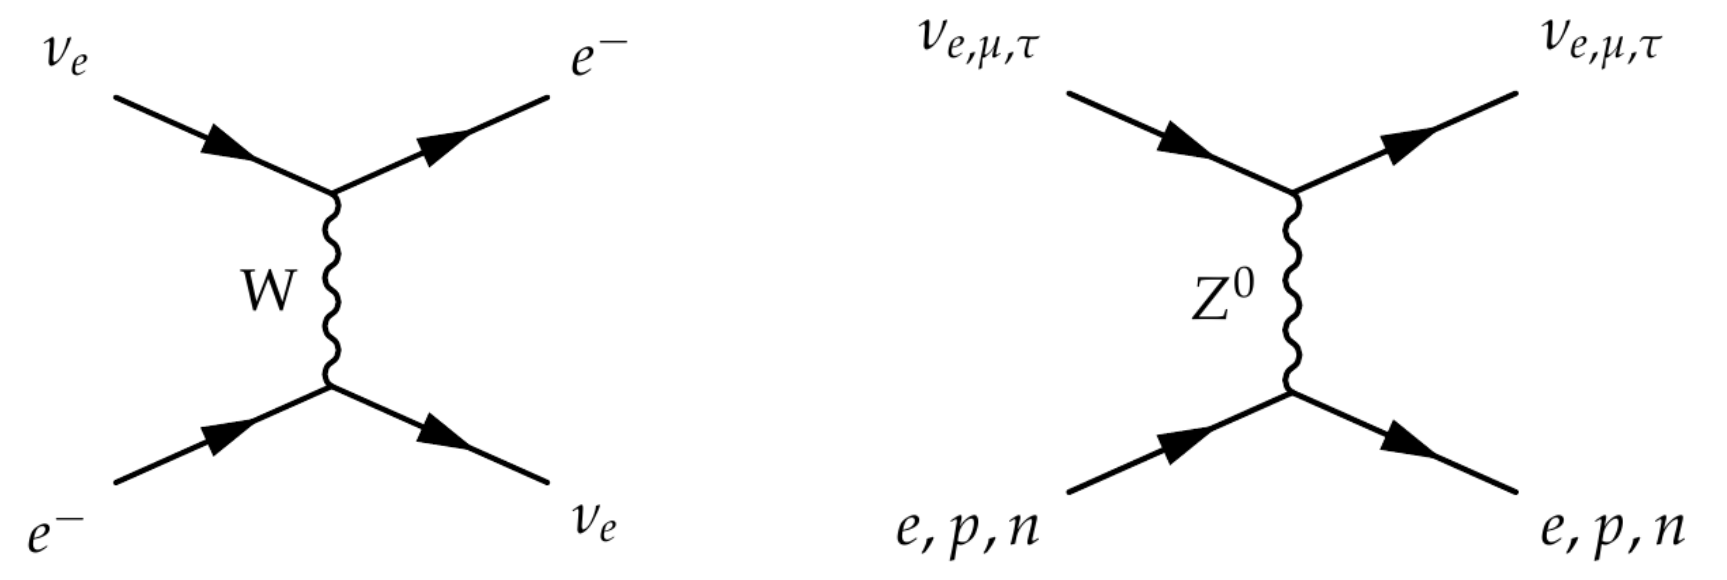
\includegraphics[width=0.8\textwidth, trim={0mm 0mm 0mm 0mm}, clip,page=1]{figures/theory/msw_effect}
%	\caption{Interaction diagrams with matter for different neutrino flavours}
%	\label{fig:msw_effect}
%\end{figure}
\begin{figure}[h]
	\begin{subfigure}[t]{0.32\textwidth}
		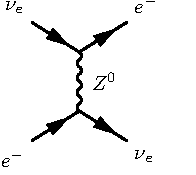
\includegraphics[width=0.8\textwidth, clip,page=1]{figures/theory/feynmp_crop}
		\caption{$\nu_e$ on $e^-$}
	\end{subfigure}
	\begin{subfigure}[t]{0.32\textwidth}
		\includegraphics[width=0.8\textwidth, clip,page=3]{figures/theory/feynmp_crop}
		\caption{$\nu_{e,\mu,\tau}$ on $e,p,n$}
	\end{subfigure}
	\begin{subfigure}[t]{0.32\textwidth}
		\includegraphics[width=0.8\textwidth, clip,page=2]{figures/theory/feynmp_crop}
		\caption{$\bar{\nu}_e$ on $e^-$}
	\end{subfigure}
	\caption{Interaction diagrams with matter for different neutrino flavours, highlighting (anti-)electron neutrino differences giving rise to different matter-effects for (anti-)electron neutrinos.}
	\label{fig:msw_effect}
\end{figure}

Electron neutrinos experience a modified Hamiltoninan potential $\Delta V = \pm 2\sqrt{2}G_F E_\nu N_e$, where $G_F$ is the Fermi constant, $E_\nu$ is the neutrino energy and $N_e$ is the electron number density of the matter, where the neutrino(anti) picks up the positive(negative) term. The effect modifies the oscillation probability to have stronger dependence on $\sin \left(\ldots \Delta m^2 \ldots \right)$, hence the sign of $\Delta m^2$ can be resolved when significant matter interactions occur\cite{msw_summary}.

\section{Neutrino Interactions}
\label{sec:theory:int}
Our limited knowledge of neutrino-matter interactions make them a dominant systematic for current long-baseline, intermediate energy neutrino oscillation experiments. The parametrisation of neutrino interaction systematics for this thesis is given in \autoref{subsec:syst_xsec}, with an overview provided here. Detailed discussions can be found in \cite{katori_martini,ulrich_review,nieves_review}.

Generally, the $E_\nu \sim 0.5-5\text{ GeV}$ regime is referred to as the ```intermediate energy region''. Neutrino-matter interactions in this region involve a range of complex nuclear physics, in which the neutrino can interact with the entire nucleus (e.g. coherent\cite{Berger_Sehgal_coh} or giant resonance\cite{crpa} interactions), nucleon pairs, single bound nucleons, and quarks (as in DIS). At the low end of the energy range, additional nuclear effects such as nucleon-nucleon correlations\cite{nieves1,nieves2}, $\Delta$ baryon in-medium modifications\cite{nuclear_effects_1pi}, $W$-boson self-energy corrections\cite{nieves1}, and nucleus spectral functions \cite{benhar}, are important. The high-end of the region is dominated by deep inelastic scattering (DIS), with dependence on parton distribution functions. The transition regions between producing no, single and multiple pions is particularly poorly modelled\cite{katori_martini,ulrich_review,nieves_review}. Neutrino-nucleus and nucleon scattering theory is often inspired by results from electron scattering experiments\cite{joanna}, such as CLAS\cite{clas} at JLAB. The electron scattering experiments have the benefit of a very narrow beam energy spectrum, so can study nuclear effects at specific $Q=P_{in}-P_{out}$ to the nucleus---unachievable with current neutrino sources.

In Monte Carlo event generators, the neutrino interaction process is commonly factorised into four parts: 1) A nucleon is simulated from a nuclear model and is used as a target for the neutrino interaction and we boost into its rest-frame, 2) The neutrino interacts with chosen nucleon which is now at rest, equivalent to a neutrino-nucleon interaction, 3) The outgoing particles from the fundamental vertex are propagated through the nucleus with radiative and final state interactions applied, 4) The particles are boosted back into the lab frame.

The total cross-sections in $E_\nu$, $\sigma(E_\nu)$, for the NEUT 5.3.3\cite{neut} generator used by T2K are shown in \autoref{fig:neut_xsecs}. At T2K energies ($E_\nu\sim0.6\text{ GeV}$) the primary interaction mode is CCQE. Charged pion production becomes important at $E_\nu\sim1\text{ GeV}$, and multi-$\pi$ and DIS above $E_\nu\sim2.5\text{ GeV}$. Since this analysis aims to minimise systematics for oscillation analyses---which select the charged-current 0$\pi$ final state at SK---the 0$\pi$ systematics have the largest impact.
\begin{figure}[h]
	\centering
	\begin{subfigure}[t]{0.42\textwidth}
		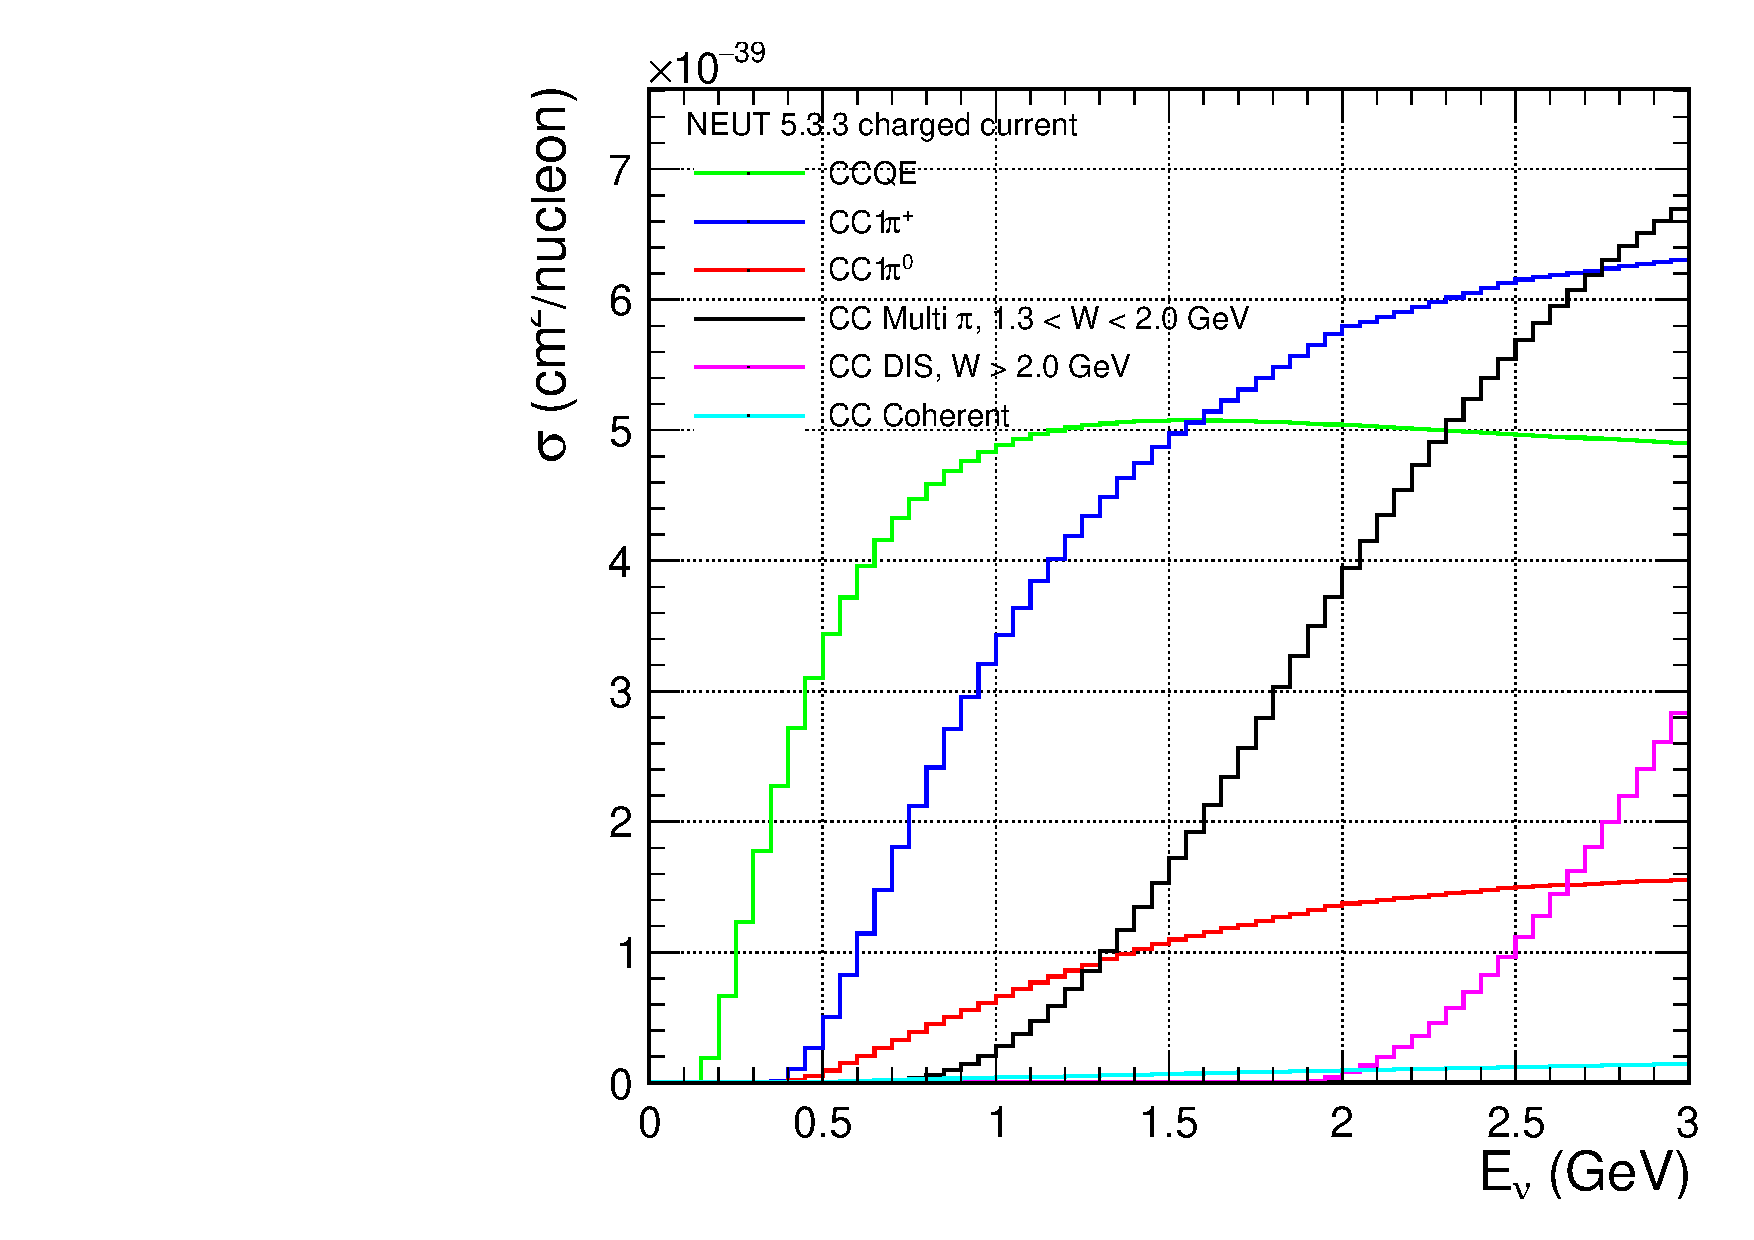
\includegraphics[width=\textwidth, trim={0mm 0mm 0mm 0mm}, clip,page=1]{figures/niwg/NEUT_533_xsecs}
		\caption{Charged current}
	\end{subfigure}
	\begin{subfigure}[t]{0.42\textwidth}
		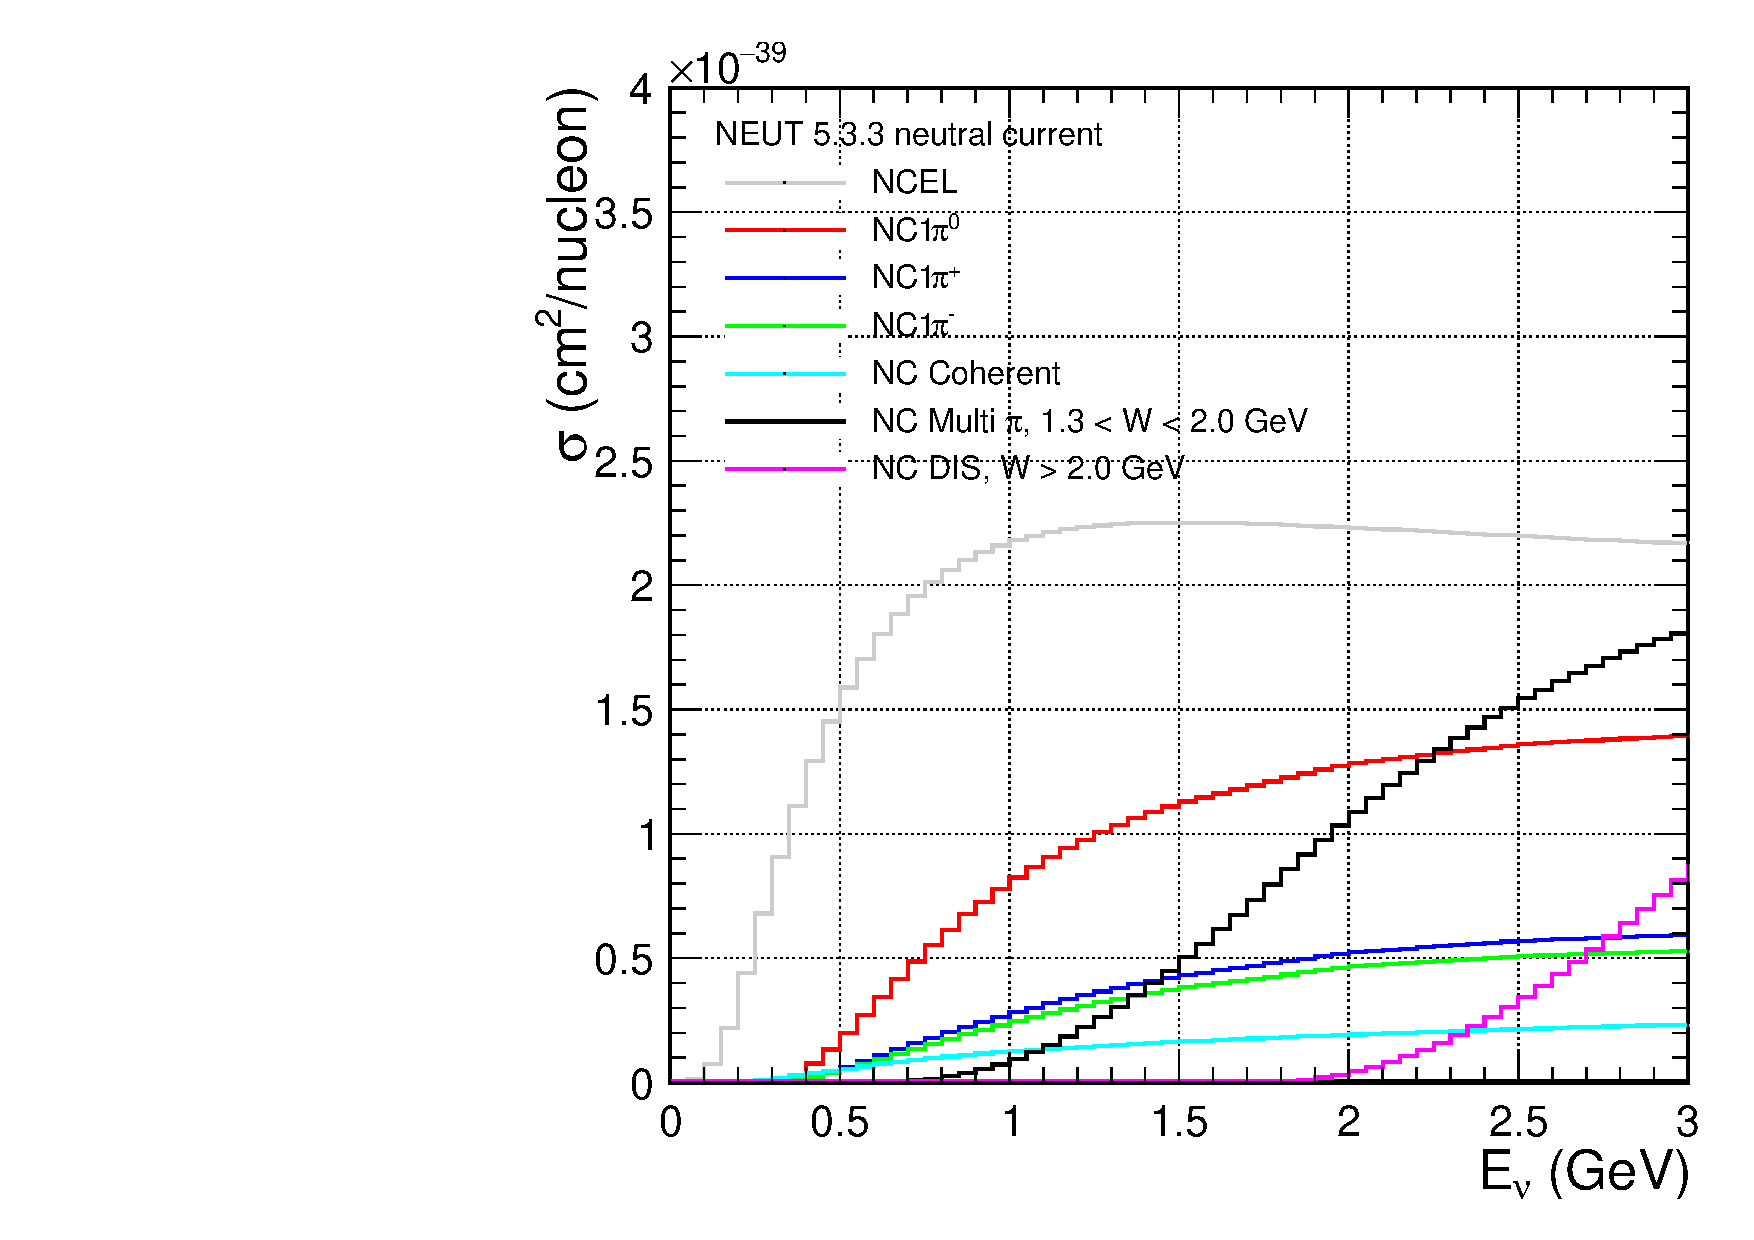
\includegraphics[width=\textwidth, trim={0mm 0mm 0mm 0mm}, clip,page=1]{figures/niwg/NEUT_533_xsecs_NC}
		\caption{Neutral current}
	\end{subfigure}
	\caption{Total cross-sections from the NEUT 5.3.3\cite{neut} neutrino interaction generator}
	\label{fig:neut_xsecs}
\end{figure}

\subsection{CC0$\pi$}
\autoref{fig:cc0pi_diag} shows some pseudo diagrams of the definition of the 0$\pi$, CCQE and one 2p2h process. The CC0$\pi$ signal definition does not include hadronic information, so the CCQE and 2p2h processes both produce 0$\pi$ final states. T2K uses the CCQE diagram for neutrino energy reconstruction, assuming a nucleon at rest. If 2p2h events are included in the selection it biases $E_\nu$, and wrongly estimating the bias has a noticeable effect on oscillation parameters. The same holds true for including single pion events due to unreconstructed pions or final state interactions.
\begin{figure}[h]
	\centering
	\begin{subfigure}[t]{0.32\textwidth}
		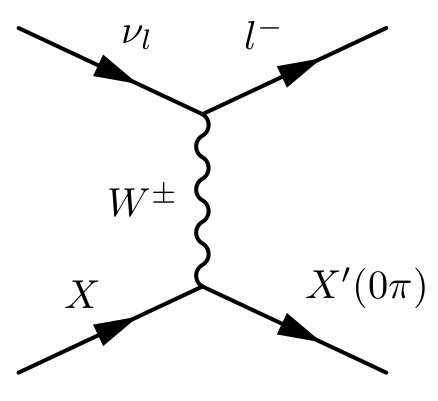
\includegraphics[width=\textwidth, trim={0mm 0mm 0mm 0mm}, clip,page=1]{figures/niwg/diagrams/CC0pi}
		\caption{CC0$\pi$, defined as having an outgoing charged lepton and no charged or neutral pions}
	\end{subfigure}
	\begin{subfigure}[t]{0.32\textwidth}
		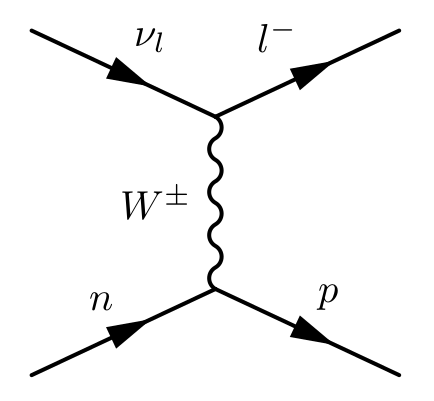
\includegraphics[width=\textwidth, trim={0mm 0mm 0mm 0mm}, clip,page=1]{figures/niwg/diagrams/CCQE}
		\caption{CCQE, defined as having interacted on an initial state neutron, producing an outgoing charged lepton and proton}
	\end{subfigure}
	\begin{subfigure}[t]{0.32\textwidth}
		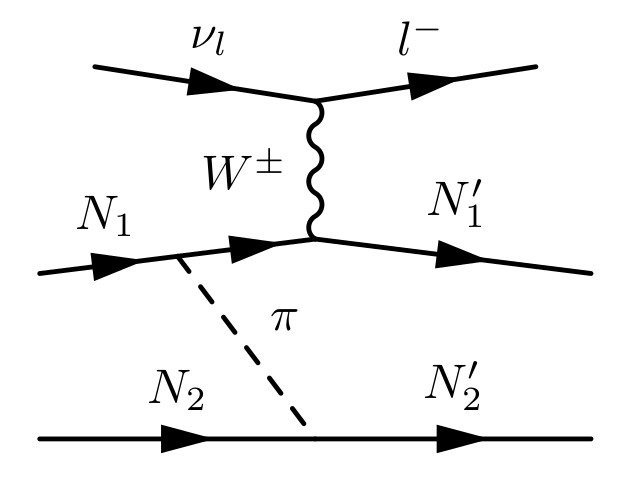
\includegraphics[width=\textwidth, trim={0mm 0mm 0mm 0mm}, clip,page=1]{figures/niwg/diagrams/2p2h_possibly}
		\caption{One of many 2p2h processes, defined as an interaction on two initial state nucleons which are coupled}
	\end{subfigure}
	\caption{CC0$\pi$, CCQE and 2p2h pseudo-diagrams}
	\label{fig:cc0pi_diag}
\end{figure}

Generally, the neutrino-nucleon CCQE interaction is relatively well understood. The current effort in the field is to understand the impact of form factor choices, numerous nuclear effects, and minimising the models' impacts on cross-section and oscillation measurements.

\subsection{Single Pion Production}
\autoref{fig:1pi_diags} shows the dominant charged-current neutrino-nucleon interactions giving rise to single pion production (SPP). The interaction proceeds by a resonant state here labelled as $\Delta$, which is dominant at T2K energies. SPP makes up $\sim20\%$ of selected 0$\pi$ events at SK due to missing pions.
\begin{figure}[h]
	\centering
	\begin{subfigure}[t]{0.32\textwidth}
		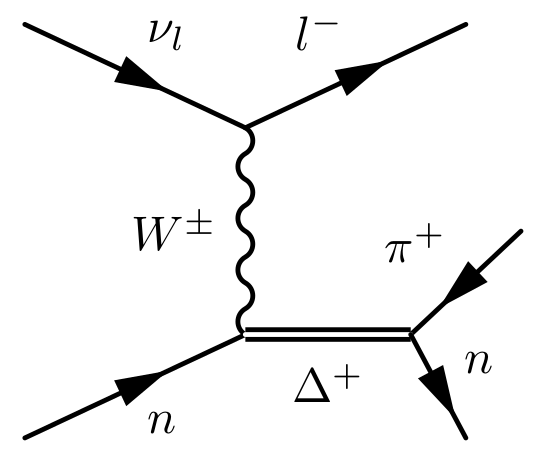
\includegraphics[width=\textwidth, trim={0mm 0mm 0mm 0mm}, clip,page=1]{figures/niwg/diagrams/CC1npip}
		\caption{CC1$\pi^+$1n}
	\end{subfigure}
	\begin{subfigure}[t]{0.32\textwidth}
		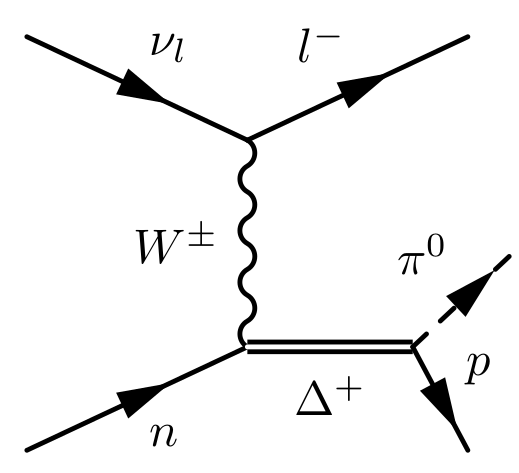
\includegraphics[width=\textwidth, trim={0mm 0mm 0mm 0mm}, clip,page=1]{figures/niwg/diagrams/CC1pi0}
		\caption{CC1$\pi^0$}
	\end{subfigure}
	\begin{subfigure}[t]{0.32\textwidth}
		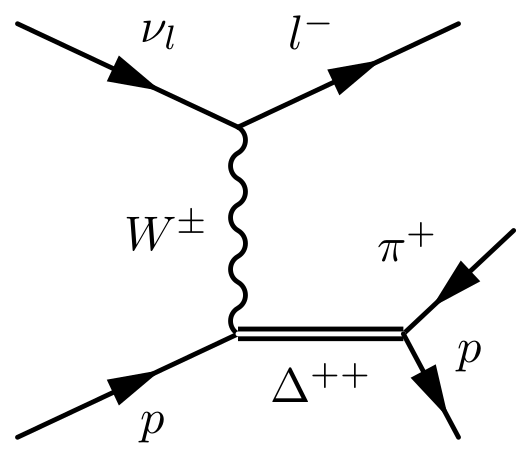
\includegraphics[width=\textwidth, trim={0mm 0mm 0mm 0mm}, clip,page=1]{figures/niwg/diagrams/CC1ppip}
		\caption{CC1$\pi^+$1p}
	\end{subfigure}
	\caption{Charged-current single pion production on a nucleon via a $\Delta$ resonance}
	\label{fig:1pi_diags}
\end{figure}

Contrary to the CCQE interaction, single pion production on free nucleons is poorly modelled. The low hadronic mass $(W)$ regime where the single $I_{3/2}$ $\Delta^{++}\rightarrow p+\pi^+$ interaction dominates can be considered understood, although resonance-resonance and resonance-non-resonance interference present at higher $W$ is not. Additionally, in-medium effects from resonance fields propagating the nucleus are poorly understood and multi-nucleon couplings often unmodelled\cite{nustec,katori_martini}.

\subsection{Multi-$\pi$ and DIS}
The transition from SPP to DIS is generally referred to as soft inelastic scattering (SIS). NEUT uses a custom interpolation between $1.3 < W < 2.0 \text{GeV}$, selecting events with $N_\pi>1$ to avoid double counting SPP cross-sections. Other generators such as GENIE\cite{genie} and NuWro\cite{NuWro} use different implementations. A pseudo diagram is shown in \autoref{fig:dis_diags}, where fragmentation causes the pion emissions.

\subsection{Subdominant Interactions}
Subdominant interactions with small interaction cross-sections can populate very specific signal regions, e.g. NC$1\gamma$ and NC1$\pi^0$ mimicking $\nu_e + X\rightarrow e^- + X'$, and differences in $\nu_e$ vs $\nu_\mu$. Historically, there is much less cross-section data on NC interactions than CC and barely any using electron neutrinos, and it is common to trust model extrapolation from CC to NC rather than test against data. 

The charged current coherent process shown in \autoref{fig:coh_diags} occupies a very specific phase space: the very forward going, collinear lepton-pion, low $Q^2$ region. This is important since it has the same final state as single pion production, although not produced through a resonance, making up about 10\% of the most forward-going \cosmu bin in CC1$\pi$ selections.
\begin{figure}[h]
	\centering
	\begin{subfigure}[t]{0.42\textwidth}
		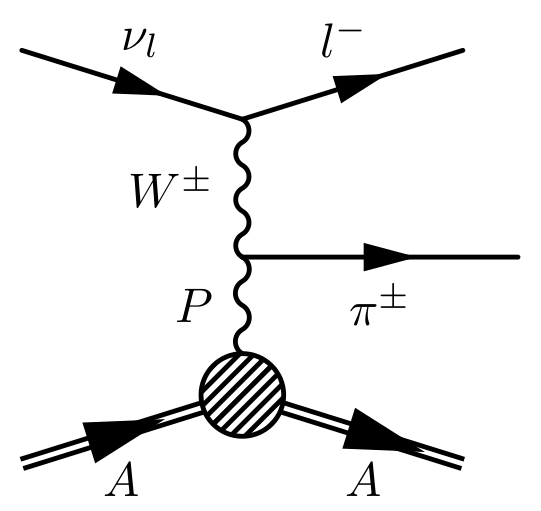
\includegraphics[width=\textwidth, trim={0mm 0mm 0mm 0mm}, clip,page=1]{figures/niwg/diagrams/CCcoh}
		\caption{CC coherent}
		\label{fig:coh_diags}
	\end{subfigure}
	\begin{subfigure}[t]{0.42\textwidth}
		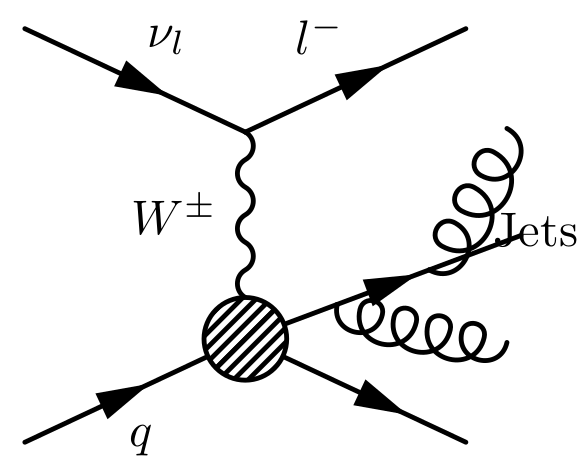
\includegraphics[width=\textwidth, trim={0mm 0mm 0mm 0mm}, clip,page=1]{figures/niwg/diagrams/CCmultipion}
		\caption{CC DIS}
		\label{fig:dis_diags}
	\end{subfigure}
	\caption{Coherent and multi-pion/DIS scattering diagrams}
	\label{fig:coh_dis_diags}
\end{figure}

\subsection{Intranuclear Hadronic Cascades}
The nuclear cascade following the initial neutrino-nucleon interaction is handled by a microscopic hadron propagation in NEUT. The hadron interaction probabilities are re-calculated as the hadron travels through the nucleus, seen in \autoref{fig:fsi_cascade}. 

Simulations can be considered to agree relatively well with pion scattering data\cite{thesis_elder}, but there are concerns that extrapolating results into the neutrino-nucleus interaction is poorly justified\cite{ulrich_review}. More sophisticated models exist in the Giessen-Boltzmann-Uehling-Uhlenbeck (GiBUU)\cite{gibuu} generator, although its role as a primary generator in neutrino physics is currently unviable due to computational requirements.
\begin{figure}[h]
	\centering
	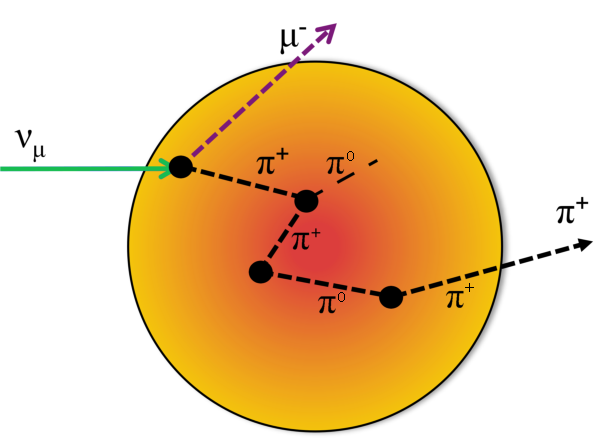
\includegraphics[width=0.3\textwidth, trim={0mm 0mm 0mm 0mm}, clip,page=1]{figures/niwg/diagrams/cascade}
	\caption{An example of a pion FSI cascade}
	\label{fig:fsi_cascade}
\end{figure}

\section{Experimental Overview}
\label{sec:exp_overview}
Neutrino oscillations is now an established physics phenomenon, cemented by awarding the 2015 Nobel Prize in Physics to Kajita-san (SK) and Art McDonald (SNO) for their experiments' measurements of solar and atmospheric neutrino oscillations. This section gives a brief introduction and overview of neutrino oscillation experiments and production mechanisms, summarised in \autoref{fig:all_neutrino_expts}. Experiments are generally categorised in neutrino energy $E$ and baseline $L$, and the combination of $L/E$ largely determines which oscillation parameter(s) an experiment has sensitivity too.
\begin{figure}[h]
	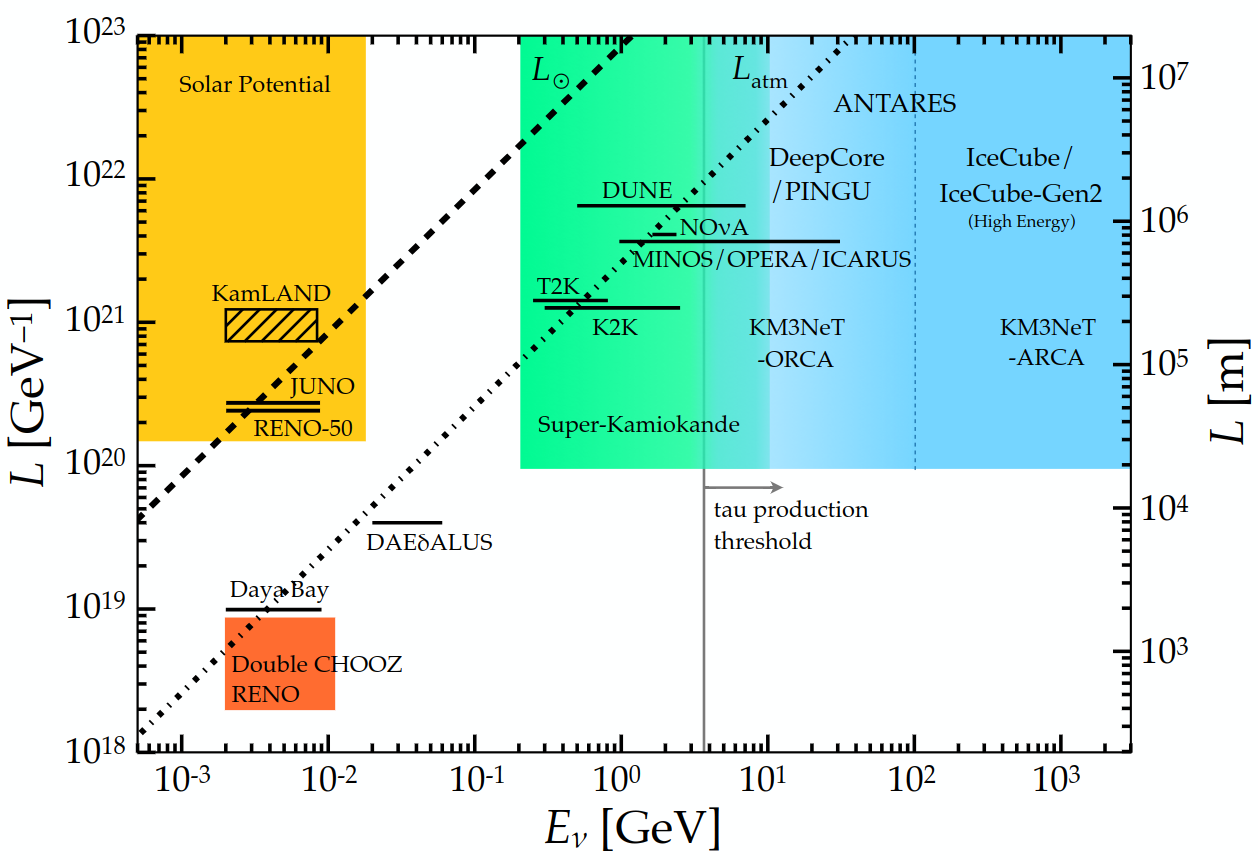
\includegraphics[width=0.7\textwidth, trim={0mm 0mm 0mm 0mm}, clip,page=1]{figures/theory/le_experiments}
	\caption{Neutrino oscillation experiments in baseline $L$ and energy $E$. Figure from \cite{ic_neutrino_2018}.}
	\label{fig:all_neutrino_expts}
\end{figure}

\subsection{Solar Neutrinos}
Solar neutrinos emanate from various nuclear fusion products and decays in the sun. \autoref{tab:solar_flux} shows the fluxes for various sources, where the $pp$ flux is strongest. However, the neutrino energy is often below threshold for the largest contributors to the flux, and most solar neutrino experiments measure the $^{8}\text{B}$ flux, shown in \autoref{fig:solar_flux}.
\begin{table}[h]
	\begin{tabular}{l | c c}
		\hline
		\hline
		Reaction & Label & Flux ($\text{cm}^{-2} \text{s}^{-1}$) \\
		\hline
		$p+p\rightarrow ^{2}\text{H} + e^+ + \nu_e$ & $pp$ & $5.95\times10^{10}$ \\
		$p+e^-+p\rightarrow ^{2}\text{H} \nu_e$ & $pep$ & $1.40\times10^{8}$ \\
		$^{3}\text{He} + p\rightarrow ^{4}\text{H} + e^+ + \nu_e$ & $hep$ & $9.3\times10^{3}$ \\
		$^{7}\text{Be} + e^- \rightarrow ^{7}\text{Li} + \nu_e$ & $^{7}\text{Be}$ & $4.77\times10^{9}$ \\
		$^{8}\text{B} \rightarrow ^{8}\text{Be}* + e^+ \nu_e$ & $^{8}\text{B}$ & $5.05\times10^{6}$ \\
		\hline
		\hline
	\end{tabular}
	\caption{Integrated solar neutrino flux from various solar processes in the $pp$ chain. Table replicated from \cite{solar_review}.}
	\label{tab:solar_flux}
\end{table}

\begin{figure}[h]
	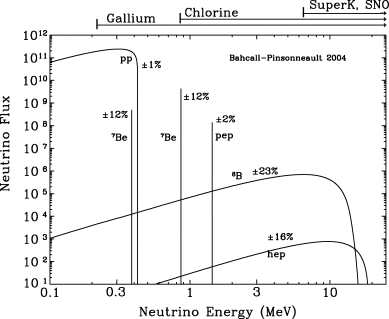
\includegraphics[width=0.5\textwidth, trim={0mm 0mm 0mm 0mm}, clip,page=1]{figures/theory/solar_flux}
	\caption{Solar flux from different solar fusion processes, including thresholds of experiments. Figure from \cite{sno_solar_flux}.}
	\label{fig:solar_flux}
\end{figure}

R. Davis and J. Bachall continued their 1964 measurements\cite{davis} of the solar neutrinos from $^{8}\text{B}$ and in 1968\cite{davis_sun} announced a solar $\nu_e$ flux a factor of seven below the expected ($\sim2\sigma$ significance), at the time attributed to inaccurate solar model calculations. This was the birth of the ``solar neutrino problem'', which Bruno Pontecorvo and Vladimir Gribov in 1969\cite{pontecorvo_gribov} proposed solving by invoking a $\nu_e\leftrightarrow\nu_\mu$ oscillation similar to $K^0 \leftrightarrow\bar{K}^0$, giving rise to the PMNS paradigm in its current form, first developed around the early 1960s. In 1989, the Kamiokande experiment\cite{kamiokande_solar} confirmed the 1968 measurements of Davis and Bachall, measuring a solar neutrino flux from $^{8}\text{B}$  of $\sim0.5$ the expected, agreeing with the higher statistics data from Homestake\cite{davis_sun2}. The solar neutrino deficit was confirmed from the low threshold detectors SAGE\cite{sage_solar} and GALLEX\cite{gallex_solar}, additionally capable of detecting $p p$ neutrinos using $^{71}\text{Ga}+\nu_e \rightarrow ^{71}\text{Ge}+e^-$.

The Sudbury Neutrino Observatory (SNO) put the nail in the coffin in 2002\cite{sno_solar} by measuring solar neutrinos from $^{8}\text{B}$ in three channels: $\nu_e + d \rightarrow p+p+e^-$ (CC), $\nu_x + d\rightarrow p+ n + \nu_x$ (NC) and $\nu_x + e^- \rightarrow \nu_x+e^-$ (ES). The measured neutrino rates had a $\nu_e$ component consistent with previous measurements, a strong non-$\nu_e$ component 5.3$\sigma$ above zero, and a NC component consistent with predictions from solar models.

Additionally, the low threshold, low background, Borexino experiment detected solar neutrinos from the $^{8}\text{B}$, $^{7}\text{Be}$, $pep$, and $pp$ processes\cite{borexino_summary}. The final stages of Borexino aims to measure the CNO cycle and the next-generation SNO+ experiment aims to confirm and improve these measurements, and make detailed measurements of the MSW effect, solar metallicity and luminosity\cite{sno_plus}.

Although the solar neutrino oscillation parameters $\Delta m^2_{21}$ and $\theta_{12}$ are considered well-constrained, there is $\sim 2\sigma$ tension on $\Delta m^2_{21}$ between the solar neutrino measurements at SK and SNO (which are internally compatible), and the long baseline reactor anti-electron-neutrino experiment, KamLAND\cite{m2_tension}, measuring the same oscillation process but with a different neutrino source.

\subsection{Atmospheric Neutrinos}
Atmospheric neutrinos are emitted when cosmic rays interact with nuclei in the earth's atmosphere, producing mesons which decay into neutrinos, amongst other particles. The primary decay is the pion decay,
\begin{gather*}
	\pi^\pm \rightarrow \mu^\pm + \nu_\mu(\bar{\nu}_\mu) \\
	\mu^\pm \rightarrow e^\pm + \bar{\nu}_\mu (\nu_\mu) + \nu_e (\bar{\nu}_e)
\end{gather*}
giving rise to a total of three neutrinos. The atmospheric neutrino flux calculations from Honda\cite{honda_flux} is shown in \autoref{fig:atmos_flux}, which peaks in the 1-10 GeV region, notably higher than the solar neutrinos.
\begin{figure}[h]
	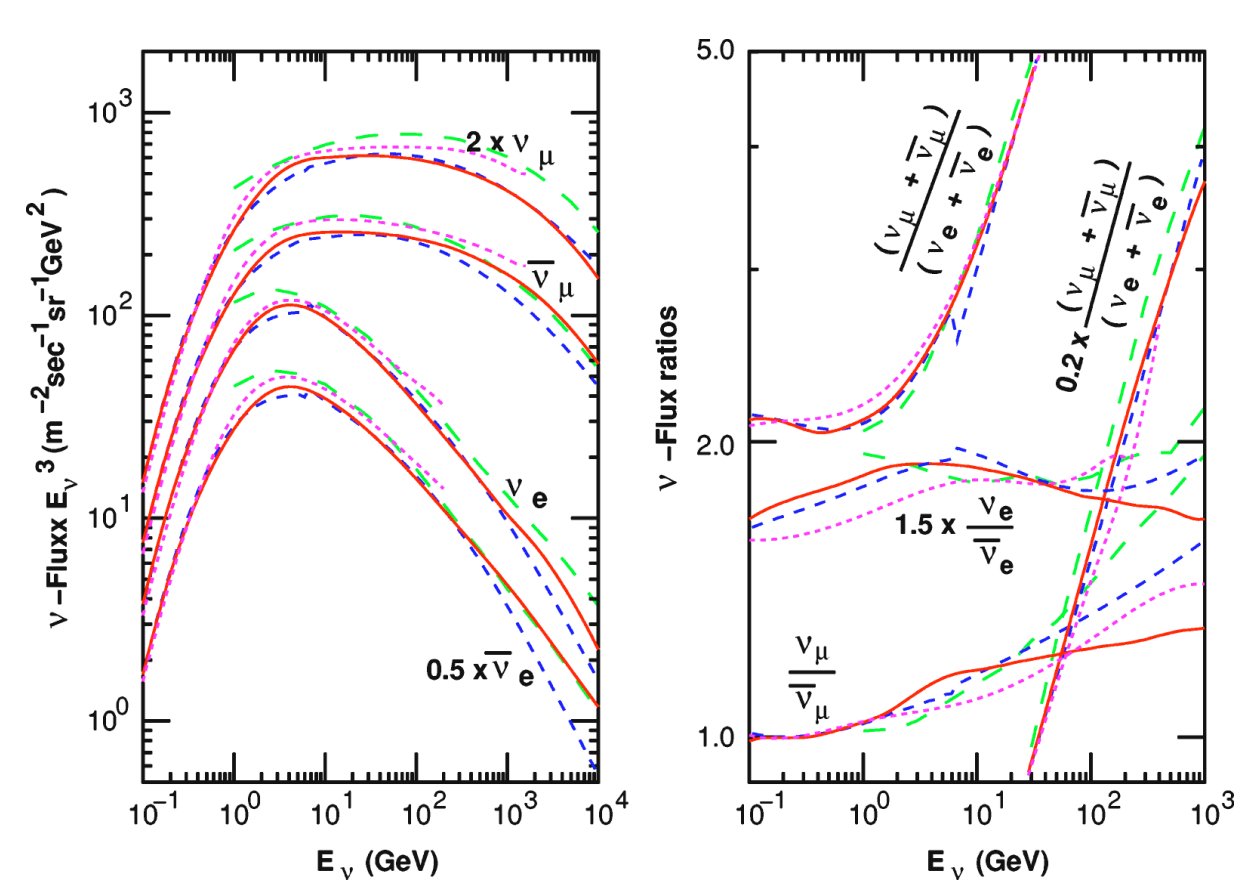
\includegraphics[width=0.7\textwidth, trim={0mm 0mm 0mm 0mm}, clip,page=1]{figures/theory/honda_flux}
	\caption{Atmospheric neutrino flux from Honda et al. \cite{honda_flux}.}
	\label{fig:atmos_flux}
\end{figure}

In 1965 F. Reines\cite{reines_atmos} and C.V. Achar\cite{india_atmos_hint} first saw hints of atmospheric $\nu_\mu$ disappearance in deep underground laboratories through $\nu_\mu(\bar{\nu}_\mu) + X \rightarrow \mu^\pm + X'$. The Irvine-Michigan-Brookhaven (IMB) experiment observed deficits of $\nu_\mu$ interactions in 1986\cite{imb}, and Kamiokande II in 1988\cite{kamiokande_atmos_hint} verified this and found muon-like events of $59\pm7\%$ the prediction, although good agreement of electron-like single-prong events. The Soudan-2 experiment\cite{soudan2} also saw muon neutrino deficiency with a flavour ratio of $0.72\pm0.19^{+0.05}_{-0.07}$ relative the expectation. 

When SK in 1998 published\cite{sk_disc} their high-statistics\footnote{4353 fully-contained and 301 partially-contained events} $\nu_\mu$ data, they found $R=\left( \mu/e \right)_\text{Data}/\left( \mu/e \right)_\text{MC} =0.65\pm0.05\pm0.08$. They additionally fitted the oscillation parameters, finding the data well described by $\nu_\mu \leftrightarrow \nu_\tau$ rather than $\nu_\mu \leftrightarrow \nu_e$ oscillations. The summary of flavour ratios for atmospheric neutrinos is seen in \autoref{fig:atmos_ratio}, where the majority of the high precision data sits at $R=0.5-0.8$.
\begin{figure}[h]
	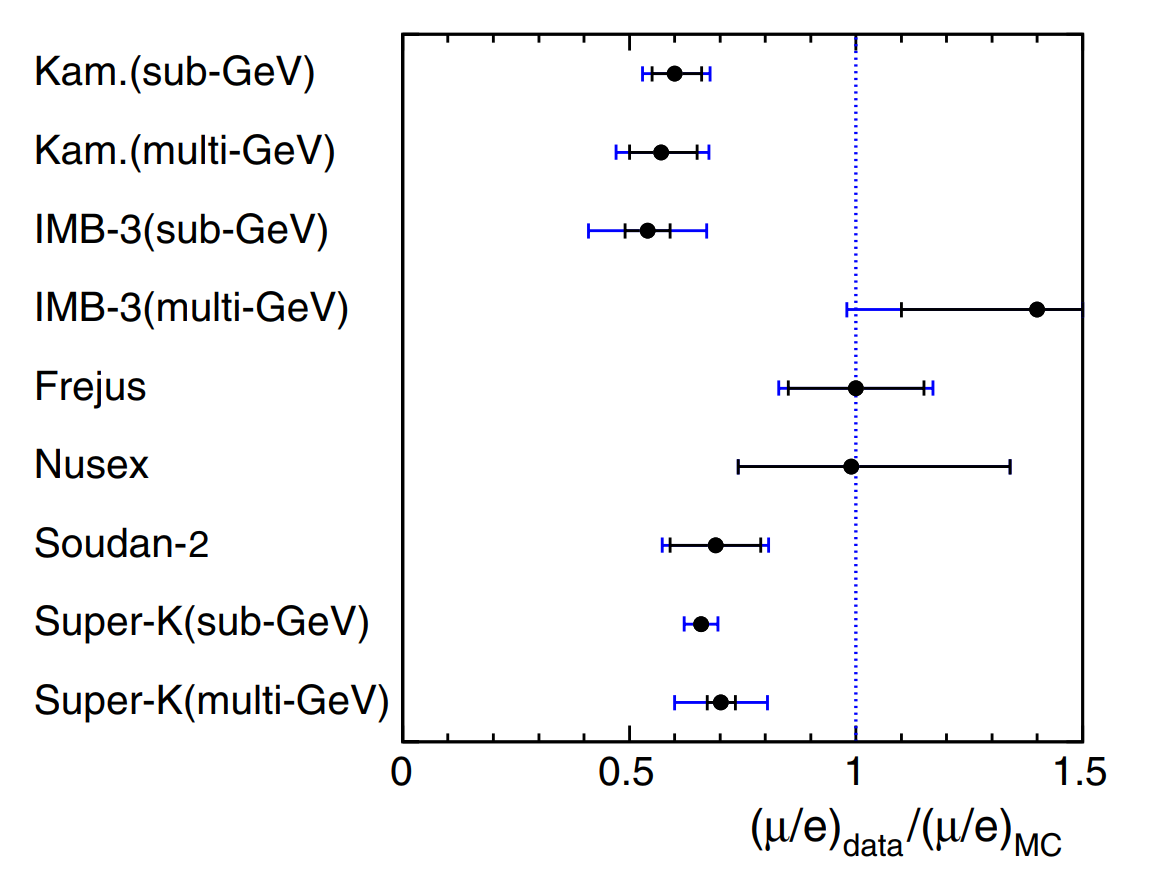
\includegraphics[width=0.7\textwidth, trim={0mm 0mm 0mm 0mm}, clip,page=1]{figures/theory/flavour_ratio}
	\caption{Measured flavour ratios for various historic atmospheric neutrino experiments, showing consistent under-prediction of the $\mu/e$ ratio in data and simulation. Figure from \cite{kajita_summary}.}
	\label{fig:atmos_ratio}
\end{figure}

Atmospheric neutrino observatories after the mid 2000s have focussed on measuring $\nu_\mu\rightarrow\nu_\mu$ with increasing precision. Furthermore, by isolating regions of specific zenith angle (and therefore baseline $L$), the extent of the matter effects are also studied, which may resolve the ordering of the mass states. This is largely the focus of the atmospheric neutrino programmes at IceCube\cite{icecube}, ANTARES\cite{antares}, SNO \cite{sno_atmos} and SK\cite{superk}. The latter has also made attempts at isolating $\nu_\tau$ events\cite{superk_tau}, claiming $4.6\sigma$ discovery of $\nu_\tau$ appearance in 2017. A summary of some recent results including complementary long baseline accelerator neutrino experiments can be seen in \autoref{fig:atmos_data}.
\begin{figure}[h]
	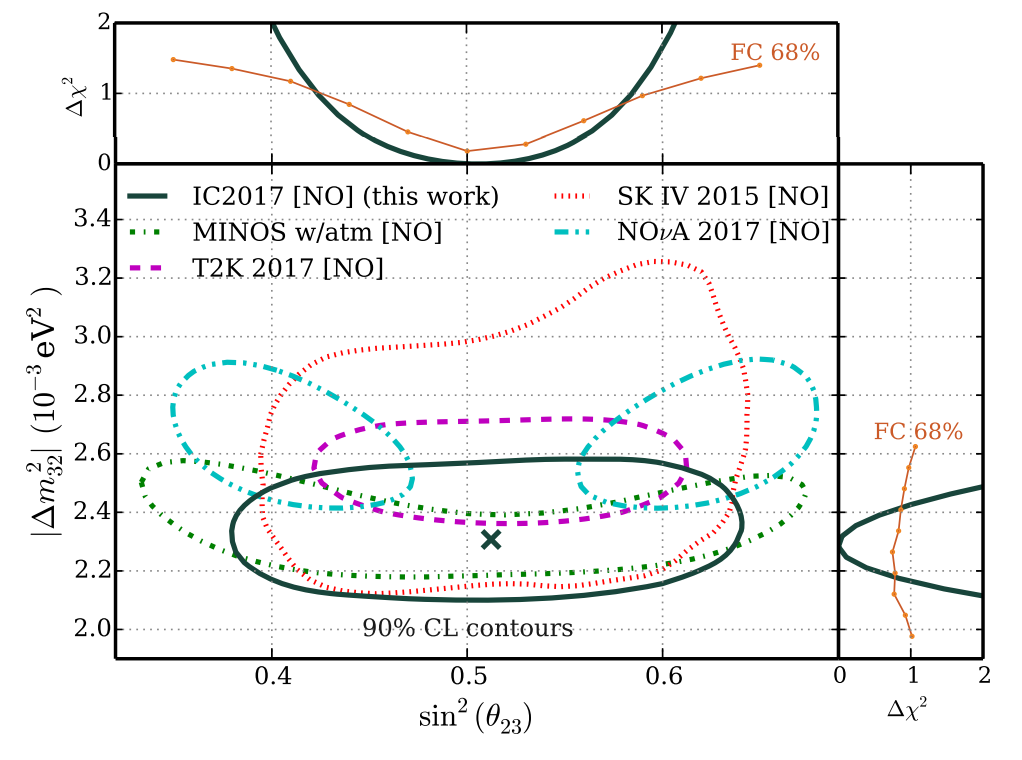
\includegraphics[width=0.7\textwidth, trim={0mm 0mm 0mm 0mm}, clip,page=1]{figures/theory/icecube_comp}
	\caption{Measured atmospheric oscillation parameters from recent atmospheric and long baseline accelerator neutrino experiments, assuming normal ordering. Figure from \cite{icecube}.}
	\label{fig:atmos_data}
\end{figure}

\subsection{Accelerator Neutrinos}
Accelerator neutrino experiments are similar to atmospheric experiments in neutrino energy, baseline and the neutrino source's production mechanism. The neutrinos are made by impinging protons from accelerators on targets, producing a flurry of mesons which typically decay into muon flavoured neutrinos, amongst others. Experiments often have the ability to deflect and/or focus mesons after the target, enabling sign selection and thus $\nu_\mu$ and $\bar{\nu}_\mu$ selection. In contrast to atmospheric neutrinos, accelerator neutrinos are about 90\% muon flavoured.

The atmospheric neutrino oscillations, outlined earlier, became the driver behind the accelerator programme in the late 1990s. Since the neutrino energy and baseline can be tuned and chosen in an accelerator experiment, the oscillation dip suggested by atmospheric neutrino experiments can be bombarded with statistics. Furthermore, the dependence on the atmospheric flux simulation is removed\cite{lbnl_review}. The disadvantage is the reduced total flux at the far-detector, generally forcing the baseline to $L<1000\text{ km}$, which limits the impact of the matter effect and sensitivity to the mass ordering. The majority of long baseline accelerator neutrino experiments include a near detector which samples the beam before any long baseline oscillations have taken place.

The short-baseline ($L\sim 1\text{ km}$) accelerator neutrino experiments, such as MiniBooNE\cite{mb_design}, MINER$\nu$A\cite{minerva_design}, and the upcoming SBND programme\cite{sbnd}, are generally intended to measure neutrino cross-sections and perform short baseline oscillation searches. They may also serve as neutrino beam monitors for other experiments. The interaction measurements are used to inform neutrino event generators\cite{neut,genie,NuWro}, aiding in informing systematic uncertainties for neutrino cross-section and oscillation experiments.

The pioneering long-baseline ($L\sim 100-1000\text{ km}$) experiments MINOS\cite{minos_obs} and K2K\cite{k2k_obs} confirmed the atmospheric neutrino mixing in $\nu_\mu \rightarrow \nu_\mu$, finding compatible oscillation parameters. The searches for $\nu_\mu \rightarrow \nu_e$ at K2K and MINOS were not statistically significant\cite{k2k_noobs,minos_disc} and were discovered by the next generation experiments T2K\cite{t2k_disc} and \nova\cite{nova_disc}, with evidence of the $\bar{\nu}_\mu \rightarrow \bar{\nu}_e$ oscillation presented by \nova at Neutrino 2018\cite{nova_neutrino2018}. The Japanese experiments K2K and T2K have consistently used the 50,000 tonne water Cherenkov detector SK\cite{superk} as the far detector, with plastic scintillator based near-detectors and a baseline of $L\sim250-300\text{ km}$ and $E\sim0.5-2\text{ GeV}$. Both MINOS and \nova, with $L\sim700\text{ km}$ and $E\sim2-5\text{ GeV}$, use(d) purpose-built functionally identical near and far-detectors, allowing for many uncertainties from systematic parameters to be reduced significantly.

In Europe, the OPERA\cite{opera} experiment was designed to look for the dominant $\nu_\mu \rightarrow \nu_\tau$ oscillation at $L\sim700\text{ km}$. The ICARUS\cite{icarus} experiment searched for $\nu_\mu\rightarrow\nu_e$ from a fourth ``sterile'' neutrino, observed by LSND\cite{lsnd} and MiniBooNE\cite{miniboone_sterile} which has been questioned by the community\cite{lsnd_refute}. The detection threshold for the charged current interaction $\nu_\tau + X \rightarrow \tau + X'$ is $E_\nu\sim 3.5\text{ GeV}$, so the neutrino beam from CERN to Gran Sasso (CNGS)\cite{cngs} was wide-band with $E_\nu = 10-25\text{ GeV}$. The $\tau$ detection requires very fine granularity and OPERA used nuclear emulsions whereas ICARUS pioneered the use of liquid argon TPCs in neutrino physics. OPERA measured $\nu_\tau$ appearance\cite{opera_final_tau} at 6.1$\sigma$, and both OPERA and ICARUS found no evidence of sterile neutrinos\cite{icarus_lsnd,opera_lsnd}.

\subsection{Reactor Anti-Electron Neutrinos}
Reactor neutrinos are formed in $\beta$ decay of fission products in nuclear reactors, e.g. $^{231}\text{Th} \rightarrow ^{231}\text{Pa} + e^- + \bar{\nu}_e$ and $^{215}\text{Po} \rightarrow ^{211}\text{Pb} + e^- + \bar{\nu}_e$. The neutrino flux depends on the relative fission yields of the products, but generally has a similar energy spectrum to solar neutrinos, in the 1-10 MeV range. The $\bar{\nu}_e$ flux from a test reactor is shown in \autoref{fig:reactor_flux}.
\begin{figure}[h]
	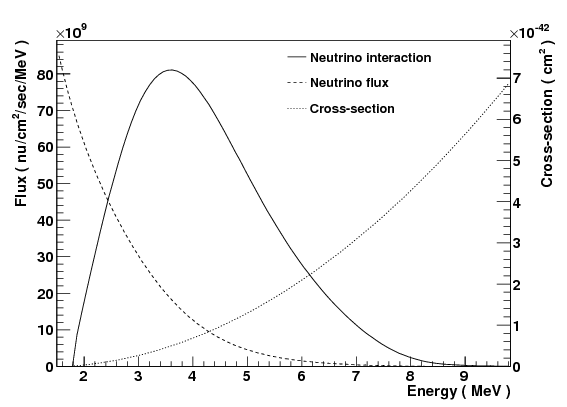
\includegraphics[width=0.6\textwidth, trim={0mm 0mm 0mm 0mm}, clip,page=1]{figures/theory/reactor_flux}
	\caption{Reactor flux for the Japanese experimental fast reactor, JOYO. Figure from \cite{reactor_flux}.}
	\label{fig:reactor_flux}
\end{figure}

Reactor anti-electron neutrinos are exclusively detected by the IBD interaction, in which the $e^+ + e^- \rightarrow 2\gamma$ annihilation photons are measured in scintillator. Many experiments additionally dope or surround the scintillator with a high neutron capture element (e.g. $^{6}\text{Li}$ or $^{157}\text{Gd}$). In the case of Gd doping, the signal consists of the prompt $2\gamma$ followed by a $\sim30\mu\text{s}$ delayed $\gamma$ cascade with $E_\gamma^{tot}\sim8\text{ MeV}$ from the Gd de-excitation, facilitating signal-background separation\cite{daya_bay,reno}.

Similar to accelerator neutrino experiments, the reactor experiments can be categorised by baseline. Short baseline experiments with $L\sim1-2\text{ km}$ perform world-leading measurements of $|\Delta m^2_{13}|$ and $\sin^2\theta_{13}$ and probe parts of the sterile neutrino spectrum. Daya Bay\cite{daya_bay_disc}, RENO\cite{reno_disc} and Double Chooz\cite{double_chooz} all measured a relatively large $\sin^2 \theta_{13}$, enabling $\nu_e$ appearance to be observed at long baseline neutrino experiments such as T2K and \nova. The short baseline reactor results on $\sin^2\theta_{13}$ are often used in atmospheric and accelerator oscillation analyses for increased sensitivity to the 2,3 parameters, the mass ordering, and $\delta_{CP}$. A summary plot of the measured neutrino oscillation parameters by short baseline reactor and long baseline accelerator neutrino oscillation experiments is shown in \autoref{fig:13_sector}.
\begin{figure}[h]
	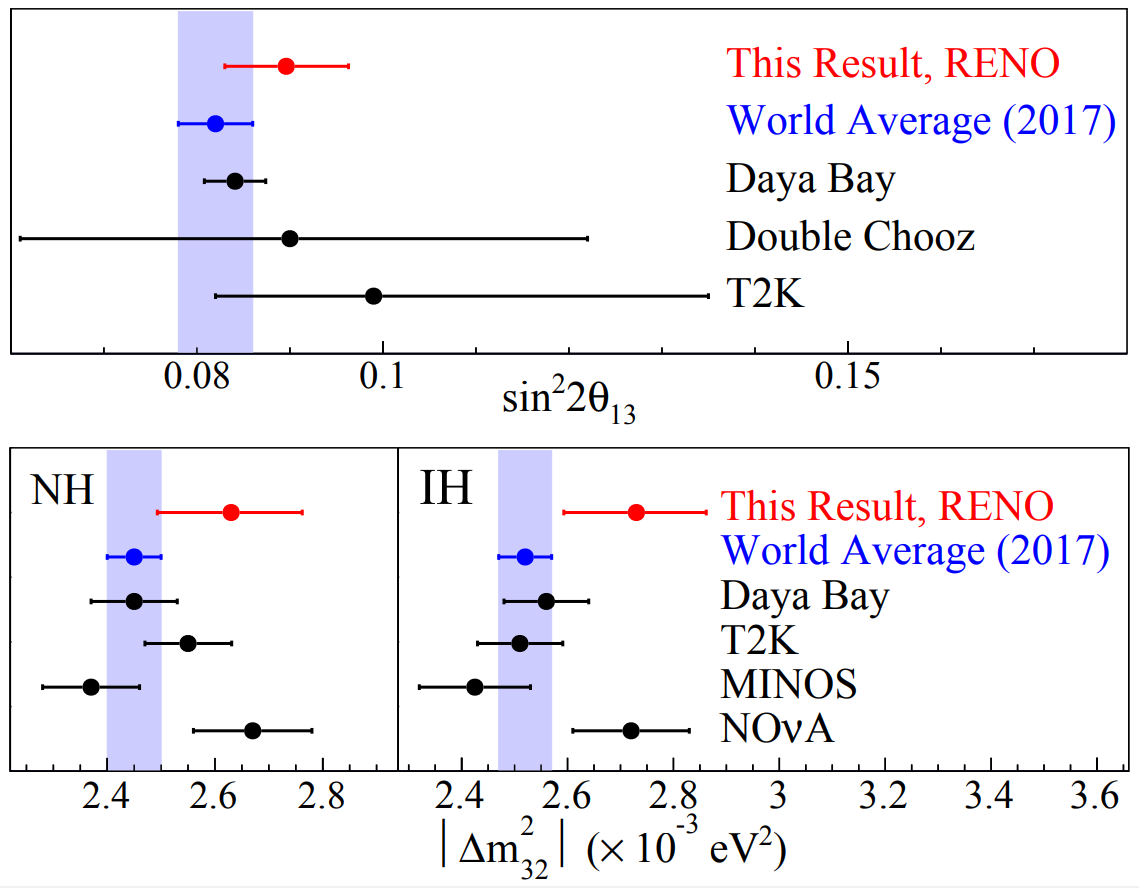
\includegraphics[width=0.6\textwidth, trim={0mm 0mm 0mm 0mm}, clip,page=1]{figures/theory/reno_theta_dm13}
	\caption{$\Delta m^2_{23}$ and $\sin^2 2\theta_{13}$ measurements from reactor (Daya Bay\cite{daya_bay}, RENO\cite{reno_new} and Double Chooz\cite{double_chooz_old}) and accelerator (T2K\cite{t2k_2015}, \nova\cite{nova_2017} and MINOS\cite{minos_numu_nue}) neutrinos. Figure from \cite{reno_new}.}
	\label{fig:13_sector}
\end{figure}

The only medium baseline experiment ($L\sim50\text{ km}$) is JUNO\cite{juno}, currently under construction in China. It aims to measure the neutrino mass ordering by separating the oscillations into fast and slow parts from $\Delta m^2_{23}$ and $\Delta m^2_{12}$, and improve measurements of $\sin^2 \theta_{12}$.

The Japanese KamLAND experiment is the only long baseline ($L\sim180\text{ km}$) reactor anti-neutrino experiment to have run. It measured $\bar{\nu}_e$s from 56 Japanese nuclear power reactors with good sensitivity to $\Delta m^2_{21}$. Additionally, combining KamLAND with SNO and SK solar data reduces uncertainties on $\Delta m^2_{21}$ and $\tan^2\theta_{12}$, as shown in \autoref{fig:21_sector}. These results are used as priors in the T2K oscillation analyses.
\begin{figure}[h]
	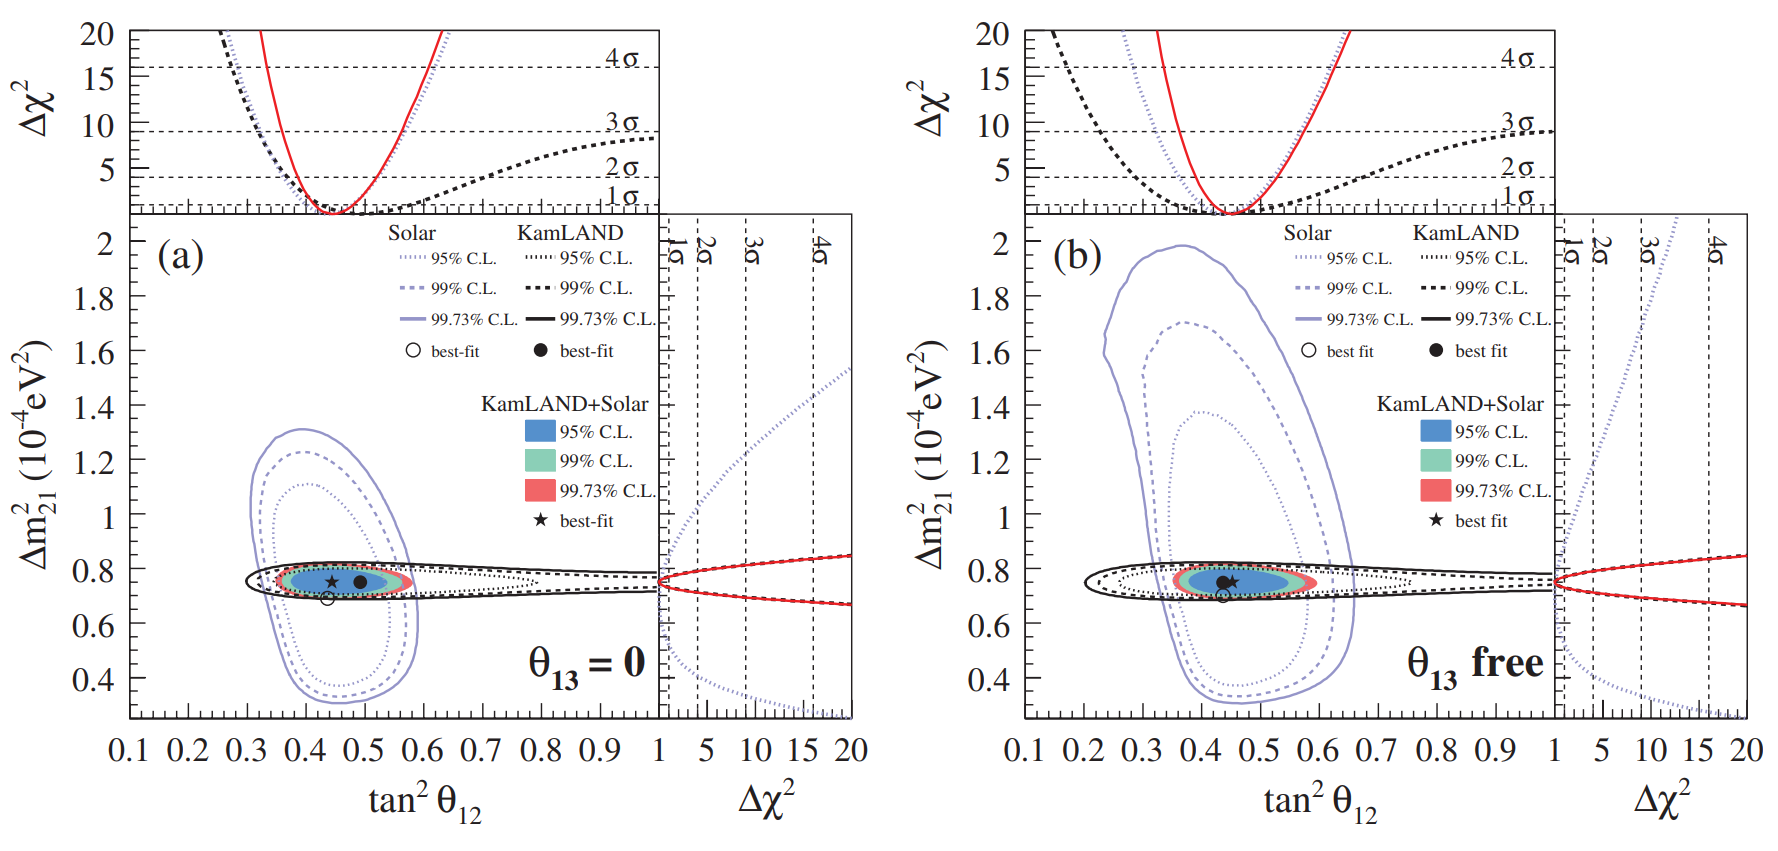
\includegraphics[width=0.7\textwidth, trim={0mm 0mm 0mm 0mm}, clip,page=1]{figures/theory/kamland_solar_comb}
	\caption{$\Delta m^2_{21}$ and $\theta_{21}$ measurements from KamLAND, SNO and SK (Solar). Figure from \cite{kamland_2011}.}
	\label{fig:21_sector}
\end{figure}

The short baseline reactor experiments at $\sim1\text{ km}$ have consistently measured neutrino event excess at $E_\nu\sim5\text{ MeV}$\cite{double_chooz, daya_bay, reno}, which is currently unresolved. The culprit is claimed to be either poor neutrino flux modelling or a sterile neutrino\cite{huber_neos,steriles}. As a result, very short baseline ($L\sim10-20\text{ m}$) experiments NEOS\cite{neos}, DANSS\cite{danss}, PROSPECT\cite{prospect}, STEREO\cite{stereo} and SoLi$\delta$\cite{solid} have been commissioned to measure $\bar{\nu}_e$ disappearance. None have found evidence of a sterile neutrino, and all have confirmed the 5 MeV excess.

  \chapter{The NEUT neutrino interaction event generator}
\label{chap:NEUT}

\section{Generator background}
\label{sec:NEUT:background}


  \chapter{The NUISANCE framework}
\label{chap:NUISANCE}

\section{Justification}
\label{chap:NUISANCE:justification}
large data-mc comparisons
compare different generators

\section{Framework structure}
\label{chap:NUISANCE:framework}

\section{Examples}
\label{chap:NUISANCE:examples}
  \chapter{Fitting NEUT single pion production}
\label{chap:1pi_fits}

\section{Background}
\label{sec:1pi_fits:background}


\section{Selecting data}
\label{sec:1pi_fits:data}


\section{Fitting}
\label{sec:1pi_fits:fit}


\section{Propagating results}
\label{sec:1pi_fits:prop}


  \chapter{Updating the single pion model}
\label{chap:1pi_update}

\section{Updating Rein-Sehgal ejection mechanism}
\label{sec:1pi_update:RS_ej}
\subsection{Theory}
\subsection{Implementation}
\subsection{Validation}
\subsection{Examples and results}
Compare to data, compare to other MC

\section{Implementing Monireh Kabirhnezhad single pion production}
\label{sec:1pi_update:Minoo}
\subsection{Theory}
\subsection{Implementation}
\subsection{Validation}
\subsection{Examples and results}
  \chapter{ND280 fits}
\label{chap:ND280}

\section{T2K}
The T2K experiment

\section{ND280}
Describe me

\section{Super-Kamiokande}

\section{T2K oscillation analysis chain overview}
The T2K oscillation analyses have a myriad of input groups providing central values and covariances for the systematic parameters. The ND280 beam group provides data on the neutrino beam, the NuMu and Nue systematics and selections groups provide ND280 systematics and suggested binning, the Neutrino Interactions Working Group (NIWG) provide neutrino interaction systematics, and the T2K-SK group provides systematics and selections for SK. Since ND280 and SK are in the same neutrino beam, the high-statistics neutrino samples at ND280 can be used to constrain the simulation prior to seeing data at SK. At the near-detector the flux model, neutrino interaction model and ND280 model is fit. Details on these systematics will be provided in \autoref{subsec:ND280:syst:xsec, subsec:ND280:syst:flux, subsec:ND280:syst:det}. 

T2K has two separate groups fitting near-detector data with the intent of maximising model likelihood: BANFF \red{INSERT ACRONYM} and MaCh3 \red{INSERT ACRONYM}. The two frameworks use identical event selections and systematic parameters, outlined below in \autoref{subsec:ND280:sel} and \autoref{subsec:ND280:syst}, but entirely different methods of evaluating the model goodness and exploring the parameter space.

BANFF interfaces to the popular gradient-descent minimizer MINUIT \red{CITE} and MaCh3 uses a custom Markov Chain Monte Carlo sampler to sample the high dimensional parameter space. Importantly, the BANFF attempts to find the global minimum of the test-statistic given the data and the model, whereas MaCh3 explores an area around the minimum test-statistic with the intent of sampling the Bayesian posterior. Therefore, MaCh3 does not necessarily locate a set of ``best-fit'' parameters with covariances assuming a parabolic minimum: instead it provides a full high-dimensional posterior with arbitrary shape. Once the model is constrained by near-detector data, the T2K oscillation analysis chain can then proceed using the model proposed by the near-detector data and model and include oscillation effects.

However, providing a high-dimensional posterior of arbitrary shape is cumbersome, so oscillation groups often use the BANFF output. MaCh3 has the advantage of a near and far detector implementation, meaning a simultaneous fit of data from both detectors can be done. This avoids assumptions on the underlying probability distribution functions of the parameters and the likelihood surface, and additionally benefits from fully correlating the models at both detectors, allowing one to affect the other as the fit proceeds.

The following sections detail the near-detector implementation of the MaCh3 framework. It also includes comparisons and validations to the BANFF framework. It finishes with the 2017 round fit to data.

\section{Need for ND280 fits}
As statistics increase at Super-Kamiokande, there is more and more need for well-controlled systematics. The T2K oscillation analysis uses \red{CITEME}

SK without constraints
Share same beam, use near detector complex

\section{Setting up the fit}



\begin{table}[htbp]
	\centering
	\begin{tabular}{ l c c c }
		\hline
                Run & Good data POT (e+19) & Generated MC POT (e+19) & Generated Sand POT (e+19) \\
		\hline
		\hline
		2a  & 3.59337    & 92.15       & 10 \\
		2w  & 4.33934    & 120.15      & 10 \\
		\hline
		3b  & 2.17273    & 44.8        & 5 \\
		3c  & 13.6447    & 263         & 25 \\
		\hline
		4a  & 17.8271    & 349.9       & 30 \\
		4w  & 16.4277    & 349.65      & 29.15 \\
		\hline
		5   & 4.3468     & 208.25      & 20 \\
		\hline
		6b  & 12.8838    & 141.03      & 40 \\
		6c  & 5.07819    & 53.21       & 15 \\
		6d  & 7.75302    & 69.41       & 20 \\
		6e  & 8.51668    & 86.72       & 23 \\
		\hline
		Total FHC & 58.00494 & 1219.65 & 109.15\\
		Total RHC & 38.57849 & 558.62  & 118 \\
		Total & 96.58343 & 1778.27 & 227.15 \\
		\hline
	\end{tabular}
	\caption{Counted and generated proton-on-targets for the T2K ND280 2017 analysis. FHC denotes Forward Horn Current (neutrino dominated mode), RHC denotes Reverse Horn Current (anti-neutrino dominated mode).}
	\label{tab:pot_2017}
\end{table}




\subsection{Selections}
\label{subsec:ND280:sel}
Selections are developed by the T2K \numu and \nue groups. \red{INSERT STUFF ON SELECTIONS}

\red{Talk about anti-neutrino binning update}

\begin{itemize}
	\item FHC $\nu_{\mu}$~CC0$\pi$ bin edges: \\
	$p$ (MeV/c): 0, 300, 400, 500, 600, 700, 800, 900, 1000, 1250, 1500, 2000, 3000, 5000, 30000 \\
	$\cos\theta$:  -1, 0.6, 0.7, 0.8, 0.85, 0.9, 0.92, 0.94, 0.96, 0.98, 0.99, 1
	\item FHC $\nu_{\mu}$~CC1$\pi$  bin edges: \\
	$p$ (MeV/c):  0, 300, 400, 500, 600, 700, 800, 900, 1000, 1250, 1500, 2000, 5000, 30000 \\
	$\cos\theta$: -1, 0.6, 0.7, 0.8, 0.85, 0.9, 0.92, 0.94, 0.96, 0.98, 0.99, 1
	\item FHC $\nu_{\mu}$~CCOther bin edges: \\
	$p$ (MeV/c): 0, 300, 400, 500, 600, 700, 800, 900, 1000, 1250, 1500, 2000, 3000, 5000, 30000 \\
	$\cos\theta$:  -1, 0.6, 0.7, 0.8, 0.85, 0.9, 0.92, 0.94, 0.96, 0.98, 0.99, 1
	\item RHC $\bar{\nu}_{\mu}$~CC 1-Track bin edges: \\
	$p$ (MeV/c): 0, 400, 500, 600, 700, 800, 900, 1100, 1400, 2000, 10000 \\
	$\cos\theta$: -1.0, 0.6, 0.7, 0.8, 0.85, 0.88, 0.91, 0.93, 0.95, 0.96, 0.97, 0.98, 0.99, 1
	\item RHC $\bar{\nu}_{\mu}$~CC N-Track bin edges: \\
	$p$ (MeV/c): 0, 700, 950, 1200, 1500, 2000, 3000, 10000 \\
	$\cos\theta$: -1.0, 0.75, 0.85, 0.88, 0.91, 0.93, 0.95, 0.96, 0.97, 0.98, 0.99, 1
	\item RHC $\nu_{\mu}$~CC 1-Track bin edges: \\
	$p$ (MeV/c): 0, 400, 600, 800, 1100, 2000, 10000 \\
	$\cos\theta$: -1.0, 0.7, 0.8, 0.85, 0.9, 0.93, 0.95, 0.96, 0.97, 0.98, 0.99, 1
	\item RHC $\nu_{\mu}$~CC N-Track bin edges: \\
	$p$ (MeV/c): 0, 500, 700, 1000, 1500, 2000, 3000, 10000 \\
	$\cos\theta$: -1.0, 0.7, 0.8, 0.85, 0.9, 0.93, 0.95, 0.96, 0.97, 0.98, 0.99, 1
\end{itemize}

Similar numbers of events are expected in both FGDs with similar kinematics, so the same binning in observed muon momentum, $p$, and cosine of the muon angle, $\cos\theta$, is used for both sets of samples.  The event selections are described in more detail in TN-212~\cite{tn_212}, TN-224~\cite{tn_224}, TN-227~\cite{tn_227}, TN-246~\cite{tn_246} and TN-248~\cite{tn_248}.

\red{INSERT reference to plots and bin merging}

\subsection{Systematics}


\subsubsection{Flux}
\label{subsec:ND280:syst:det}
The flux systematics are evaluated by varying underlying parameters in the flux model and using NA61/SHINE \red{CITE} data. [7] N. Antoniou et al. CERN-SPSC-2006-034, 2006.

The NA61 data comes from runs using the thin target, whereas the T2K target is roughly 2 interaction lenghts. The data is $\pi^\pm$, $K^\pm$, $K^0_S$ and $\rho^+$.

HARP data used for pion rescattering.

Talk about the corrections in psyche
\begin{itemize}
  \item ND280 FHC $\nu_\mu$:\\
    $E_\nu^{true}$: 0, 0.4, 0.5, 0.6, 0.7, 1, 1.5, 2.5, 3.5, 5, 7, 30 \\

  \item ND280 FHC $\bar{\nu}_\mu$:\\
    $E_\nu^{true}$: 0, 0.7, 1, 1.5, 2.5, 30 \\

  \item ND280 FHC $\nu_e$:\\
    $E_\nu^{true}$: 0, 0.5, 0.7, 0.8, 1.5, 2.5, 4, 30 \\

  \item ND280 FHC $\bar{\nu}_e$:\\
    $E_\nu^{true}$: 0, 2.5, 30 \\

  \item ND280 RHC $\nu_\mu$:\\
    $E_\nu^{true}$: 0, 0.7, 1, 1.5, 2.5, 30 \\

  \item ND280 RHC $\bar{\nu}_\mu$:\\
    $E_\nu^{true}$: 0, 0.4, 0.5, 0.6, 0.7, 1, 1.5, 2.5, 3.5, 5, 7, 30 \\

  \item ND280 RHC $\nu_e$:\\
    $E_\nu^{true}$: 0, 2.5, 30 \\

  \item ND280 RHC $\bar{\nu}_e$:\\
    $E_\nu^{true}$: 0, 0.5, 0.7, 0.8, 1.5, 2.5, 4, 30 \\

  \item SK FHC $\nu_\mu$:\\
    $E_\nu^{true}$: 0, 0.4, 0.5, 0.6, 0.7, 1, 1.5, 2.5, 3.5, 5, 7, 30 \\

  \item SK FHC $\bar{\nu}_\mu$:\\
    $E_\nu^{true}$: 0, 0.7, 1, 1.5, 2.5, 30 \\

  \item SK FHC $\nu_e$:\\
    $E_\nu^{true}$: 0, 0.5, 0.7, 0.8, 1.5, 2.5, 4, 30 \\

  \item SK FHC $\bar{\nu}_e$:\\
    $E_\nu^{true}$: 0, 2.5, 30 \\

  \item SK RHC $\nu_\mu$:\\
    $E_\nu^{true}$: 0, 0.7, 1, 1.5, 2.5, 30 \\

  \item SK RHC $\bar{\nu}_\mu$:\\
    $E_\nu^{true}$: 0, 0.4, 0.5, 0.6, 0.7, 1, 1.5, 2.5, 3.5, 5, 7, 30 \\

  \item SK RHC $\nu_e$:\\
    $E_\nu^{true}$: 0, 2.5, 30 \\

  \item SK RHC $\bar{\nu}_e$:\\
    $E_\nu^{true}$: 0, 0.5, 0.7, 0.8, 1.5, 2.5, 4, 30\\
\end{itemize}


\subsection{Detector systematics}
\label{subsec:ND280:syst:flux}
The treatment of detector systematic uncertainties is unchanged from TN-230~\cite{tn_230}, Section 3.1, page 26.
The number of detector systematics still decreased slightly from 580 to 556 due to merging bins with similar detector systematic effects for the rebinned samples.
All the consecutive bins with similar systematic values have been merged in order to reach a lower number of parameters (556) while the number of bins in the fit increased a lot (1624 bins), keeping the number of parameters under control.
It has been demonstrated with Asimov fits, the results of which are shown in \autoref{fig:2017_rebin_asimov}, that the effect of this rebinning was small.

The effect of changing the ND280 systematics binning was done with an older cross-section model than which the fit was completed in. This was due to a late delivery of the cross-section model \red{write an appendix on this model}. The flux parameters were entirely consistent.
\begin{table}
	\centering
	\begin{tabular}{ l c c }
		Parameter & Fit binning & Similar syst. merge \\
		\hline
		FSI INEL LO & $0.0 \pm 0.202$ & $0.0\pm0.200$ \\
		FSI INEL HI & $0.0 \pm 0.235$ & $0.0\pm0.233$ \\
		FSI PI PROD & $0.0 \pm 0.347$ & $0.0\pm0.344$ \\
		FSI CEX LO  & $0.0 \pm 0.416$ & $0.0\pm0.412$ \\
		FSI CEX HI  & $0.0 \pm 0.193$ & $0.0\pm0.191$ \\
		$M_A^{QE}$  & $1.2 \pm 0.0517$ & $1.2\pm0.0512$ \\
		$p_F^{C}$   & $217 \pm 36.96$ & $217\pm36.021$ \\
		2p2h norm C & $100 \pm 30.79$ & $100\pm30.56$ \\
		$E_B^{C}$   & $25.0 \pm 8.57$ & $25.0\pm8.56$ \\
		$p_F^{O}$   & $225 \pm 57.61$  & $225\pm56.16$ \\
		2p2h norm O & $100 \pm 277.98$ & $0.0\pm272.62$ \\
		$E_B^{C}$   & $27.0 \pm 9.00$ & $27.0\pm9.00$ \\
		$C_5^A$		& $1.01 \pm 0.066$ & $1.01\pm0.064$ \\
		$M_A^{1\pi}$ & $0.95 \pm 0.060$ & $0.95\pm0.059$ \\
		$I_{1/2}$ non-res & $1.30 \pm 0.180$ & $1.30\pm0.180$ \\
		CC $\nu_e$ norm & $1.00 \pm 0.030$ & $1.00\pm0.030$ \\
		DIS Shape	& $0.00 \pm 0.208$ & $0.0\pm0.208$ \\
		CC Coherent norm & $1.0 \pm 0.258$ & $1.0\pm0.257$ \\
		NC Coherent norm & $1.0 \pm 0.299$ & $1.0\pm0.299$ \\
		NC Other & $1.0 \pm 0.182$ & $1.0\pm0.181$ \\
		2p2h $\bar{\nu}$ & $1.0 \pm 0.332$ & $1.0\pm0.329$ \\
	\end{tabular}
	\caption{Cross-section parameter results from comparisons using fit binning and a merged binning for the 2015 cross-section model.}
\label{fig:2017_rebin_asimov}
\end{table}

The merged systematics binning was improved to:
\begin{itemize}
	\item FHC $\nu_{\mu}$~CC0$\pi$ bin edges: \\
	$p$ (MeV/c): 0, 1000, 1250, 2000, 3000, 5000, 30000 \\
	$\cos\theta$:  -1, 0.6, 0.7, 0.8, 0.85,0.94, 0.96, 1
	\item FHC $\nu_{\mu}$~CC1$\pi$  bin edges: \\
	$p$ (MeV/c):  0, 300, 1250, 1500, 5000, 30000 \\
	$\cos\theta$: -1, 0.7, 0.85, 0.9, 0.92, 0.96, 0.98, 0.99, 1
	\item FHC $\nu_{\mu}$~CCOther bin edges: \\
	$p$ (MeV/c): 0, 1500, 2000, 3000, 5000, 30000 \\
	$\cos\theta$:  -1, 0.8, 0.85, 0.9, 0.92, 0.96, 0.98, 0.99, 1
	\item RHC $\bar{\nu}_{\mu}$~CC 1-Track bin edges: \\
	$p$ (MeV/c): 0, 400, 900, 1100, 2000, 10000 \\
	$\cos\theta$:  -1, 0.6, 0.7, 0.88, 0.95, 0.97, 0.98, 0.99, 1.00
	\item RHC $\bar{\nu}_{\mu}$~CC N-Track bin edges: \\
	$p$ (MeV/c):  0, 700, 1200, 1500, 2000, 3000, 10000 \\
	$\cos\theta$: -1, 0.85, 0.88, 0.93, 0.98, 0.99, 1.00
	\item RHC $\nu_{\mu}$~CC 1-Track bin edges: \\
	$p$ (MeV/c):  0, 400, 800, 1100, 2000, 10000 \\
	$\cos\theta$:   -1, 0.7, 0.85, 0.90, 0.93, 0.96, 0.98, 0.99, 1.00
	\item RHC $\nu_{\mu}$~CC N-Track bin edges: \\
	$p$ (MeV/c):  0, 1000, 1500, 2000, 3000, 10000 \\
	$\cos\theta$: -1, 0.8, 0.90, 0.93, 0.95, 0.96, 0.97, 0.99, 1.00
\end{itemize}

\subsubsection{Cross-section}
\label{subsec:ND280:syst:xsec}
splines vs normalisation parameter, Maybe extra bit on BeRPA because of involvement

\subsection{Building the Monte-Carlo prediction}
The fit proceeds by binning events in the two reconstructed muon variables $p_\mu$ and $\cos\theta_\mu$. The muon variables are chosen primarily due to excellent detector resolution of muons, and also because \sk analyses are performed in these variables. There is ongoing effort to bin in pion variables when such are present (e.g. for CC$1\pi^+$ or CCOther selections), and composite variables in the plane transverse to the neutrino. The fit uses the reconstructed variables for data and MC and does not unfold into true space.

Inspecting the POT table in \autoref{tab:pot_2017}, MC is generated with POT $\sim\times10$ data POT to avoid uncertainty from Monte Carlo statistics. To build the nominal distribution equivalent for comparison to data a number of weights are applied:
\begin{itemize}
	\item \textbf{POT weight:} \\
	A run-by-run scaling factor taking the ratio of total good flagged data to the generated Monte-Carlo POT. An event receives a one-time weight depending on what run it was from and how much MC was generated in the production. These numbers can be read off directly from \autoref{tab:pot_2017}. \\ 
	\item \textbf{Flux weight:} \\
	A run-by-run correction to the nominal neutrino flux which the production was made in. The weight is applied as a function of $E_\nu^{true}$ \red{show example of this, psycheND280utils/data/tuned13av2}, detailed in \autoref{subsec:ND280:syst:det}. An event receives a weight depending on what run it was from and it's $E_\nu^{true}$. \\
	\item \textbf{Cross-section weight:} \\
	An event-by-event weight taking the full generated event through the neutrino interaction simulation again, calculating a weight to apply to the event. The weight can be described as $w=\sigma(\textbf{x'})/\sigma(\textbf{x})$ for the neutrino interaction systematic parameter set $\textbf{x}$. The event may receive a normalisation and a shape parameter depending on its interaction type and the interaction model considered for the analysis. For example, for this analysis a $\nu_\mu$ 2p2h event on Carbon would receive both a normalisation parameter weight (2p2h Carbon) and a shape parameter weight (2p2h shape C), whereas a CC coherent event on Carbon would recieve only a normalisation weight (CC Coherent C). \\
	\item \textbf{Detector weight:} \\
	\item \textbf{Detector covariance weight:} \\
	\item \textbf{Beam covariance weight:} \\
\end{itemize}

\subsection{Defining the test-statistic}


\subsection{Parameters of interest}
flux and cross-section

\subsection{Fitting method: MCMC}
tests

\section{Nominal model}

\begin{table}[htbp]
	\centering
	\begin{tabular}{ l c c }
		\hline
		Sample & Data & \nd~pre-fit MC prediction \\ \hline
		\hline
		FGD1 $\nu_{\mu}$ CC0$\pi$ ($\nu$ mode)                  & 17136 & 16724    \\% \hline
		FGD1 $\nu_{\mu}$ CC1$\pi$ ($\nu$ mode)                  & 3954  & 4381  \\% \hline
		FGD1 $\nu_{\mu}$ CC Other ($\nu$ mode)                  & 4149  & 3944  \\% \hline
		\hline
		FGD1 $\bar{\nu}_{\mu}$ CC 1-Track ($\bar{\nu}$ mode)    & 3527 & 3588  \\% \hline
		FGD1 $\bar{\nu}_{\mu}$ CC N-Tracks ($\bar{\nu}$ mode)   & 1054 & 1067  \\% \hline
		\hline
		FGD1 $\nu_{\mu}$ CC 1-Track ($\bar{\nu}$ mode)          & 1363 & 1272   \\% \hline
		FGD1 $\nu_{\mu}$ CC N-Tracks ($\bar{\nu}$ mode)         & 1370 & 1357   \\% \hline
		\hline
		FGD2 $\nu_{\mu}$ CC0$\pi$ ($\nu$ mode)                  & 17443 & 16959 \\% \hline
		FGD2 $\nu_{\mu}$ CC1$\pi$ ($\nu$ mode)                  & 3366  & 3564  \\% \hline
		FGD2 $\nu_{\mu}$ CC Other ($\nu$ mode)                  & 4075  & 3571  \\% \hline
		\hline
		FGD2 $\bar{\nu}_{\mu}$ CC 1-Track ($\bar{\nu}$ mode)    & 3732 &  3618  \\% \hline
		FGD2 $\bar{\nu}_{\mu}$ CC N-Tracks ($\bar{\nu}$ mode)   & 1026 &  1077  \\% \hline
		\hline
		FGD2 $\nu_{\mu}$ CC 1-Track ($\bar{\nu}$ mode)          & 1320 & 1263  \\% \hline
		FGD2 $\nu_{\mu}$ CC N-Tracks ($\bar{\nu}$ mode)         & 1253 & 1247  \\% \hline
		\hline
		\hline
		Total & 64768 & 63633 \\
		\hline
		\hline
		FHC POT & $58.00\times10^{19}$ & $1219.65\times10^{19}$  \\% \hline
		RHC POT & $38.58\times10^{19}$ & $558.62\times10^{19}$   \\% \hline
	\end{tabular}
	\caption{Observed and predicted event rates for the different \nd~samples in the BANFF/MaCh3 fits. N.B. the MC rates are rounded to nearest integer in this table, for higher precision see \autoref{tab:eventrate}.}
	\label{tab:event_rates}
\end{table}

\begin{sidewaystable}
	\resizebox{\textwidth}{!}{
		\begin{tabular}{| c | c | c | c | c | c | c | c | c | c | c | c |}
			\hline
			Sample & Data  & Raw MC & POT only & POT+flux & POT+xsec & POT+det & POT + flux + xsec & POT + flux + det & POT + flux + xsec + det & MaCh3 & (BANFF-MaCh3)/BANFF \\ \hline
			FGD1 CC0$\pi$ &  17136.00 &  337436.00 &  16090.83 &  17535.92 &  15340.11 &  15905.24 &  16748.19 &  17333.49 &  16723.69 & 16723.8 & -6.60E-6 \\ \hline
			FGD1 CC1$\pi$ &  3954.00 &  84982.00 &  4058.36 &  4606.61 &  3819.31 &  4011.58 &  4352.83 &  4553.49 &  4381.48 & 4381.47 & 2.28E-6\\ \hline
			FGD1 CCOther &  4149.00 &  65286.00 &  3107.04 &  3703.69 &  3078.52 &  3071.21 &  3673.94 &  3660.96 &  3943.95 & 3943.95 & 0.00E0\\ \hline
			FGD1 Anu-CCQE &  3527.00 &  54419.00 &  3773.79 &  3881.64 &  3430.04 &  3744.02 &  3527.03 &  3851.02 &  3587.65 & 3587.77 & -3.34E-5\\ \hline
			FGD1 Anu-CCNQE &  1054.00 &  15392.00 &  1065.20 &  1101.04 &  986.32 &  1056.80 &  1021.05 &  1092.37 &  1066.91 & 1066.91 & 0.00E0\\ \hline
			FGD1 Nu-CCQE &  1363.00 &  18146.00 &  1255.92 &  1340.43 &  1194.72 &  1246.03 &  1275.92 &  1329.88 &  1272.17 & 1272.17 & 0.00E0\\ \hline
			FGD1 Nu-CCNQE &  1370.00 &  17156.00 &  1190.94 &  1316.59 &  1172.13 &  1181.54 &  1297.36 &  1306.21 &  1357.45 & 1357.45 & 0.00E0 \\ \hline
			FGD2 CC0$\pi$ &  17443.00 &  345467.00 &  16449.22 &  17921.83 &  15749.71 &  16259.57 &  17189.12 &  17715.02 &  16959.19 & 16959.3 & -6.49E-6 \\ \hline
			FGD2 CC1$\pi$ &  3366.00 &  70444.00 &  3356.97 &  3820.22 &  3190.10 &  3318.26 &  3644.01 &  3776.14 &  3564.23 & 3564.23 & 0.00E0\\ \hline
			FGD2 CCOther &  4075.00 &  63402.00 &  3018.22 &  3595.45 &  2995.68 &  2983.43 &  3572.61 &  3553.98 &  3570.95 & 3570.94 & 2.80E-6 \\ \hline
			FGD2 Anu-CCQE &  3732.00 &  55732.00 &  3864.24 &  3978.31 &  3506.34 &  3833.73 &  3608.17 &  3946.91 &  3618.27 & 3618.29 & -5.53E-6 \\ \hline
			FGD2 Anu-CCNQE &  1026.00 &  15808.00 &  1096.81 &  1134.09 &  1024.77 &  1088.15 &  1061.38 &  1125.14 &  1077.24 & 1077.24 & 0.00E0 \\ \hline
			FGD2 Nu-CCQE &  1320.00 &  18052.00 &  1241.02 &  1324.16 &  1189.64 &  1231.24 &  1269.94 &  1313.72 &  1262.63 & 1262.63 & 0.00E0 \\ \hline
			FGD2 Nu-CCNQE &  1253.00 &  16339.00 &  1136.62 &  1256.01 &  1121.38 &  1127.64 &  1240.99 &  1246.09 &  1246.71 & 1246.71 & 0.00E0 \\ \hline
			Total &  64768.00 &  1178061.00 &  60705.16 &  66516.01 &  57798.77 &  60058.44 &  63482.54 &  65804.42 &  63632.53 & 63632.9 & -5.81E-6 \\ \hline
		\end{tabular}
	}
	\caption{Event rates broken by type of weight applied for BANFF with a comparison to MaCh3. N.B. ``POT+flux+xsec+det'' is the final BANFF prediction.}
	\label{tab:eventrate}
\end{sidewaystable}

\section{Asimov results}


\subsection{Prior and posterior predictive}

\subsection{LLH scan and 1 sigma variations}

\section{Datafit results}

\subsection{Results}

\subsection{Statistical analysis}

\subsection{Compatibility}

\section{Validating to BANFF}

\section{Impact on SK oscillation analyses}

  \chapter{Updating the ND280 fit for the future}

\section{Adding run 7 and 8 data}

\begin{table}[htbp]
	\centering
	\begin{tabular}{ l c c c c }
		\hline
		Run & Good Data POT (e+19) & Generated MC POT (e+19) & Generated Sand POT (e+19) \\
		\hline
		\hline
		2a  & 3.59337    & 92.3937     & 3.7132  \\
		2w  & 4.33765    & 120.341     & 4.00035 \\
		\hline
		3b  & 2.1705     & 44.7864     & 2.35053 \\
		3c  & 13.6398    & 263.227     & 13.1337 \\
		\hline
		4a  & 17.8271    & 349.96      & 17.4125 \\
		4w  & 16.4277    & 226.216     & 15.9801 \\
		\hline
		5   & 4.3468     & 229.627     & 9.07403 \\
		\hline
		6b  & 12.7301    & 141.74      & 25.9187 \\
		6c  & 5.07819    & 52.7562     & 10.4626 \\
		6d  & 7.75302    & 68.83       & 15.8059 \\
		6e  & 8.51429    & 85.9439     & 17.2691 \\
		\hline
		7   & 24.3683	 & 337.059     & 50.3961 \\
		\hline
		8a  & 41.4909	 & 363.054	   & 40.1875 \\
		8w  & 15.8053    & 264.115 	   & 16.1263 \\
		\hline
		Total FHC & 115.29232 & 1724.0931 &  112.09418 \\
		Total RHC & 62.791 	  & 915.9561  &  127.92643 \\
		Total 	  & 178.08332 & 2640.0492 &  240.83061 \\
		\hline
		x2017 FHC   & 1.9876 \\
		x2017 RHC   & 1.6276 \\
		x2017 Total & 1.8438 \\
	\end{tabular}
	\caption{Counted and generated proton-on-targets for the T2K ND280 2018+ analysis. FHC denotes Forward Horn Current (neutrino dominated mode), RHC denotes Reverse Horn Current (anti-neutrino dominated mode).}
	\label{tab:pot_2017}
\end{table}


\begin{table}[htbp]
	\centering
	\begin{tabular}{ l c c }
		\hline
		Sample & Data & \nd~pre-fit MC prediction \\ \hline
		\hline
		FGD1 $\nu_{\mu}$ CC0$\pi$ ($\nu$ mode)                  & 33553 & 31529.2    \\% \hline
		FGD1 $\nu_{\mu}$ CC1$\pi$ ($\nu$ mode)                  & 7757  & 7997.52  \\% \hline
		FGD1 $\nu_{\mu}$ CC Other ($\nu$ mode)                  & 8068  & 6793.45  \\% \hline
		\hline
		FGD2 $\nu_{\mu}$ CC0$\pi$ ($\nu$ mode)                  & 17443 & 31732.1 \\% \hline
		FGD2 $\nu_{\mu}$ CC1$\pi$ ($\nu$ mode)                  & 6133  & 6418.42  \\% \hline
		FGD2 $\nu_{\mu}$ CC Other ($\nu$ mode)                  & 7664  & 6562.61  \\% \hline
		\hline
		FGD1 $\bar{\nu}_{\mu}$ CC0$\pi$ ($\nu$ mode)            & 6368 & 6370.47    \\% \hline
		FGD1 $\bar{\nu}_{\mu}$ CC1$\pi$ ($\nu$ mode)            & 535  & 533.342  \\% \hline
		FGD1 $\bar{\nu}_{\mu}$ CC Other ($\nu$ mode)            & 1032 & 1023.3  \\% \hline
		\hline
		FGD2 $\bar{\nu}_{\mu}$ CC0$\pi$ ($\nu$ mode)            & 6451 & 6283.55    \\% \hline
		FGD2 $\bar{\nu}_{\mu}$ CC1$\pi$ ($\nu$ mode)            & 465  & 483.358  \\% \hline
		FGD2 $\bar{\nu}_{\mu}$ CC Other ($\nu$ mode)            & 8068 & 944.017  \\% \hline
		\hline
		FGD1 RHC $\nu_{\mu}$ CC0$\pi$ ($\nu$ mode)              & 2707 & 2500.77  \\% \hline
		FGD1 RHC $\nu_{\mu}$ CC1$\pi$ ($\nu$ mode)              & 847  & 845.922 \\% \hline
		FGD1 RHC $\nu_{\mu}$ CC Other ($\nu$ mode)              & 1015 & 800.914  \\% \hline
		\hline
		FGD2 RHC $\nu_{\mu}$ CC0$\pi$ ($\nu$ mode)              & 2648 & 2554.46  \\% \hline
		FGD2 RHC $\nu_{\mu}$ CC1$\pi$ ($\nu$ mode)              & 693  & 670.813  \\% \hline
		FGD2 RHC $\nu_{\mu}$ CC Other ($\nu$ mode)              & 932  & 785.661 \\% \hline
		Total & 121432 & 114830 \\
		Total x2017 & 1.87 & 1.80 \\
		\hline
	\end{tabular}
	\caption{Observed and predicted event rates for the different \nd~samples in the MaCh3 fits. N.B. the MC rates are rounded to nearest integer in this table, for higher precision see \autoref{tab:eventrate}.}
	\label{tab:detailed_eventrate_2018}
\end{table}
BASED ON /tmp/ts-out.Md7erS on heppc205 7 apr


\begin{table}[htbp]
	\centering
	\begin{tabular}{ l c c }
		\hline
		Sample & Data & \nd~pre-fit MC prediction \\ \hline
		\hline
		FGD1 $\nu_{\mu}$ CC0$\pi$ ($\nu$ mode)                  & 33553 & 31530.5    \\% \hline
		FGD1 $\nu_{\mu}$ CC1$\pi$ ($\nu$ mode)                  & 7757  & 7997.96  \\% \hline
		FGD1 $\nu_{\mu}$ CC Other ($\nu$ mode)                  & 8068  & 6793.11  \\% \hline
		\hline
		FGD2 $\nu_{\mu}$ CC0$\pi$ ($\nu$ mode)                  & 17443 & 31736.7 \\% \hline
		FGD2 $\nu_{\mu}$ CC1$\pi$ ($\nu$ mode)                  & 6133  & 6419.23  \\% \hline
		FGD2 $\nu_{\mu}$ CC Other ($\nu$ mode)                  & 7664  & 6563.14  \\% \hline
		\hline
		FGD1 $\bar{\nu}_{\mu}$ CC0$\pi$ ($\nu$ mode)            & 6368 & 6371.09    \\% \hline
		FGD1 $\bar{\nu}_{\mu}$ CC1$\pi$ ($\nu$ mode)            & 535  & 533.187  \\% \hline
		FGD1 $\bar{\nu}_{\mu}$ CC Other ($\nu$ mode)            & 1032 & 1023.2  \\% \hline
		\hline
		FGD2 $\bar{\nu}_{\mu}$ CC0$\pi$ ($\nu$ mode)            & 6451 & 6284.65    \\% \hline
		FGD2 $\bar{\nu}_{\mu}$ CC1$\pi$ ($\nu$ mode)            & 465  & 483.469  \\% \hline
		FGD2 $\bar{\nu}_{\mu}$ CC Other ($\nu$ mode)            & 8068 & 944.175  \\% \hline
		\hline
		FGD1 RHC $\nu_{\mu}$ CC0$\pi$ ($\nu$ mode)              & 2707 & 2497.71  \\% \hline
		FGD1 RHC $\nu_{\mu}$ CC1$\pi$ ($\nu$ mode)              & 847  & 860.675 \\% \hline
		FGD1 RHC $\nu_{\mu}$ CC Other ($\nu$ mode)              & 1015 & 797.499  \\% \hline
		\hline
		FGD2 RHC $\nu_{\mu}$ CC0$\pi$ ($\nu$ mode)              & 2648 & 2553.51  \\% \hline
		FGD2 RHC $\nu_{\mu}$ CC1$\pi$ ($\nu$ mode)              & 693  & 679.99  \\% \hline
		FGD2 RHC $\nu_{\mu}$ CC Other ($\nu$ mode)              & 932  & 792.166 \\% \hline
		Total & 121432 & 114862 \\
		Total x2017 & 1.87 & 1.80 \\
		\hline
	\end{tabular}
	\caption{Observed and predicted event rates for the different \nd~samples in the BANFF/MaCh3 fits. N.B. the MC rates are rounded to nearest integer in this table, for higher precision see \autoref{tab:eventrate}.}
	\label{tab:detailed_eventrate_2018}
\end{table}
Based on full matrix /tmp/ts-out/hAdNOT heppc205 8 Apr


Based on final matrix /tmp/ts-out.86tzSy on hepp105 8Apr
FGD1 numuCC 0pi                    33553     31529.3   593.559   |     
FGD1 numuCC 1pi                    7757      7998.1    200.965   |     
FGD1 numuCC other                  8068      6793.68   376.623   |     
FGD2 numuCC 0pi                    33462     31734     613.019   |     
FGD2 numuCC 1pi                    6133      6419.04   201.759   |     
FGD2 numuCC other                  7664      6562.75   339.344   |     
FGD1 anti-numuCC 0pi               6368      6371.34   202.958   |     
FGD1 anti-numuCC 1pi               535       533.253   26.3027   |     
FGD1 anti-numuCC other             1102      1023.36   44.7771   |     
FGD2 anti-numuCC 0pi               6451      6283.35   221.72    |     
FGD2 anti-numuCC 1pi               465       483.508   22.4051   |     
FGD2 anti-numuCC other             1032      943.956   61.3131   |     
FGD1 NuMuBkg CC0pi in AntiNu Mode  2707      2485.51   82.6989   |     
FGD1 NuMuBkg CC1pi in AntiNu Mode  847       855.911   28.7885   |     
FGD1 NuMuBkg CCother in AntiNu Mode1015      804.647   58.6913   |     
FGD2 NuMuBkg CC0pi in AntiNu Mode  2648      2553.51   88.5485   |     
FGD2 NuMuBkg CC1pi in AntiNu Mode  693       679.99    38.5698   |     
FGD2 NuMuBkg CCother in AntiNu Mode932       792.166   41.2255   |     
Total                              121432    114847    3243.27   | 

Sample                             Binned    Unbinned
FGD1 numuCC 0pi                    33553     33615
FGD1 numuCC 1pi                    7757      7774
FGD1 numuCC other                  8068      8139
FGD2 numuCC 0pi                    33462     33543
FGD2 numuCC 1pi                    6133      6159
FGD2 numuCC other                  7664      7734
FGD1 anti-numuCC 0pi               6368      6380
FGD1 anti-numuCC 1pi               535       536
FGD1 anti-numuCC other             1102      1110
FGD2 anti-numuCC 0pi               6451      6464
FGD2 anti-numuCC 1pi               465       465
FGD2 anti-numuCC other             1032      1046
FGD1 NuMuBkg CC0pi in AntiNu Mode  2707      2728
FGD1 NuMuBkg CC1pi in AntiNu Mode  847       852
FGD1 NuMuBkg CCother in AntiNu Mode1015      1030
FGD2 NuMuBkg CC0pi in AntiNu Mode  2648      2667
FGD2 NuMuBkg CC1pi in AntiNu Mode  693       697
FGD2 NuMuBkg CCother in AntiNu Mode932       946
Total:                             121432    121885

Events by mode:
CCQE                720451
CC1pi               393646
CCcoh               45278
CCMpi               153787
CCDIS               190313
NC1pi0              3593
NC1pipm             15172
NCcoh               537
NCoth               55607
2p2h                116771
NC1gam              21

from /tmp/ts-out.uV5Ksu /tmp/ts-out.86tzSy on heppc105 (using v6 matrix)
\begin{sidewaystable}
  \resizebox{\textwidth}{!}{%
    \begin{tabular}{| l | c | c | c | c | c | c | c | c |}
      Sample  & MC  & POT  & Flux  & Xsec & Det & ND280 Cov & Beam Cov  & All \\
      \hline
      FGD1 numuCC 0pi & 470176 & 31464.6 & 34153.7 & 30106.3 & 30298 & 31487.9 & 31464.6 & 31529.3\\
      FGD1 numuCC 1pi & 119835 & 8059.92 & 9106.99 & 7496.3 & 7690.07 & 7959.59 & 8059.92 & 7998.1 \\
      FGD1 numuCC other & 92630 & 6224.1 & 7389.73 & 6096.03 & 5917.31 & 6144.95 & 6224.1 & 6793.68 \\

      FGD2 numuCC 0pi & 471140 & 31215.4 & 33881.4 & 30017.8 & 30361.4 & 31198.7 & 31215.4 & 31734 \\
      FGD2 numuCC 1pi & 95498 & 6303.05 & 7148.91 & 5919.55 & 6121.38 & 6184.34 & 6303.05 & 6419.04 \\
      FGD2 numuCC other & 87931 & 5839.17 & 6933.53 & 5723.31 & 5697.16 & 5773.49 & 5839.17 & 6562.75 \\

      FGD1 anti-numuCC 0pi & 96602 & 6784.14 & 6983.08 & 6247.83 & 6723.77 & 6794.13 & 6784.14 & 6371.34 \\
      FGD1 anti-numuCC 1pi & 9133 & 639.595 & 658.426 & 536.293 & 623.687 & 635.372 & 639.595 & 533.253 \\
      FGD1 anti-numuCC other & 15046 & 1066.91 & 1113.12 & 1012.08 & 1044.37 & 1055.12 & 1066.91 & 1023.36 \\

      FGD2 anti-numuCC 0pi & 95597 & 6692.82 & 6897.34 & 6185.55 & 6578.7 & 6715.93 & 6692.82 & 6283.35 \\
      FGD2 anti-numuCC 1pi & 8165 & 568.917 & 587.274 & 491.61 & 553.376 & 557.22 & 568.917 & 483.508 \\
      FGD2 anti-numuCC other & 13849 & 970.796 & 1015.05 & 927.283 & 954.657 & 961.134 & 970.796 & 943.956 \\

      FGD1 NuMuBkg CC0pi in AntiNu Mode & 34950 & 2457.88 & 2646.97 & 2392.37 & 2379.95 & 2449.2 & 2457.88 & 2485.51 \\
      FGD1 NuMuBkg CC1pi in AntiNu Mode & 12352 & 871.792 & 952.669 & 814.909 & 838.532 & 871.141 & 871.792 & 855.911 \\
      FGD1 NuMuBkg CCother in AntiNu Mode & 10894 & 764.374 & 854.448 & 750.775 & 733.571 & 764.374 & 764.374 & 804.647 \\

      FGD2 NuMuBkg CC0pi in AntiNu Mode & 35180 & 2458.01 & 2645.96 & 2408.41 & 2419.07 & 2458.01 & 2458.01 & 2553.51 \\
      FGD2 NuMuBkg CC1pi in AntiNu Mode & 9714 & 676.737 & 740.521 & 632.743 & 662.563 & 676.737 & 676.737 & 679.99 \\
      FGD2 NuMuBkg CCother in AntiNu Mode & 10421 & 732.441 & 819.628 & 718.565 & 720.726 & 732.441 & 732.441 & 792.166 \\
      \hline
      Total & 1689110 & 113791 & 124529 & 108478 & 110318 & 113420 & 113420 & 114847 \\
      

    \end{tabular}
        }
        \caption{Event rates broken by type of weight applied}
  \label{tab:detailed_eventrate_2018}
\end{sidewaystable}




\subsection{Rebinning}
The T2K run 7 and run 8 data took \red{INSERT POT} protons on target in 2015 and 2016. Run 7 was a anti-neutrino dominated run (reverse horn current, or RHC) and run 8 was a neutrino dominated run (forward horn current, or FHC). Comparing to previous runs used in analyses (run 2 to 6), run 7 and 8 roughly doubled the amount of data in both neutrino and anti-neutrino selections. \red{insert table from psyche}
% % % % % % % % % % % % % % % % % %
% FIT BINNING

\begin{itemize}
  \item FGD1 and FGD2 CC0$\pi$: 841 fit bins\\
    $p_\mu$ (MeV/c) = 0., 200., 300., 400., 450., 500., 550., 600., 650., 700., 750., 800., 850., 900., 950., 1000., 1050., 1100., 1200., 1300., 1400., 1500., 1600., 1700., 1800., 2000., 2500., 3000., 5000., 30000. \\
    $\cos\theta_\mu$ = -1., 0.5, 0.6, 0.7, 0.76, 0.78, 0.8, 0.83, 0.85, 0.88, 0.89, 0.9, 0.91, 0.92, 0.925, 0.93, 0.935, 0.94, 0.945, 0.95, 0.955, 0.96, 0.965, 0.97, 0.975, 0.98, 0.985, 0.99, 0.995, 1.\\

  \item FGD1 and FGD2 CC1$\pi$: 288 fit bins\\
    $p_\mu$ (MeV/c) = 0., 300., 350., 400., 500., 600., 650., 700., 750., 800., 900., 1000., 1100., 1200., 1500., 2000., 3000., 5000., 30000. \\
    $\cos\theta_\mu$ = -1., 0.6, 0.7, 0.8, 0.85, 0.88, 0.9, 0.92, 0.93, 0.94, 0.95, 0.96, 0.97, 0.98, 0.99, 0.995, 1. \\

  \item FGD1 and FGD2 CCOther: 342 fit bins\\
    $p_\mu$ (MeV/c) = 0., 300., 400., 500., 600., 650., 700., 750., 800., 900., 1000., 1100., 1250., 1500., 1750., 2000., 3000., 5000., 30000. \\
    $\cos\theta_\mu$ = -1., 0.6, 0.7, 0.76, 0.8, 0.85, 0.88, 0.89, 0.9, 0.91, 0.92, 0.93, 0.94, 0.95, 0.96, 0.97, 0.98, 0.99, 0.995, 1. \\

  \item FGD1 and FGD2 CC0$\pi$ RHC: 306 fit bins\\
    $p_\mu$ (MeV/c) = 0., 300., 400., 500., 550., 600., 650., 700., 750., 800., 900., 1000., 1100., 1200., 1500., 2000., 4000., 30000.\\
    $\cos\theta_\mu$ = -1., 0.6, 0.7, 0.8, 0.85, 0.9, 0.92, 0.93, 0.94, 0.95, 0.96, 0.965, 0.97, 0.975, 0.98, 0.985, 0.99, 0.995, 1.\\

  \item FGD1 and FGD2 CC1$\pi$ RHC: 48 fit bins \\
    $p_\mu$ (MeV/c) = 0., 500., 700., 900., 1300., 2500., 30000.\\
    $\cos\theta_\mu$ = -1, 0.7, 0.8, 0.9, 0.94, 0.96, 0.98, 0.99, 1\\

  \item FGD1 and FGD2 CCOther RHC: 80 fit bins \\
    $p_\mu$ (MeV/c) = 0., 600., 800., 1000., 1250., 1500., 2000., 4000., 30000.\\
    $\cos\theta_\mu$ = -1., 0.7, 0.8, 0.85, 0.9, 0.93, 0.95, 0.97, 0.98, 0.99, 1.\\

  \item FGD1 and FGD2 CC0$\pi$ $\nu$ RHC: 120 fit bins \\
    $p_\mu$ (MeV/c) = 0., 300., 500., 700., 800., 900., 1250., 1500., 2000., 4000., 30000.\\
     $\cos\theta_\mu$ = -1., 0.7, 0.8, 0.85, 0.88, 0.9, 0.92, 0.94, 0.96, 0.97, 0.98, 0.99, 1.\\

   \item FGD1 and FGD2 CC1$\pi$ $\nu$ RHC: 40 fit bins \\
     $p_\mu$ (MeV/c) = 0., 600., 800., 1500., 30000.\\
      $\cos\theta_\mu$ = -1, 0.7, 0.8, 0.86, 0.9, 0.94, 0.96, 0.97, 0.98, 0.99, 1\\

    \item FGD1 and FGD2 CCOther $\nu$ RHC: 80 fit bins \\
      $p_\mu$ (MeV/c) = 0., 600., 1000., 1250., 2000., 4000., 30000.;\\
       $\cos\theta_\mu$ = -1., 0.7, 0.8, 0.86, 0.9, 0.93, 0.95, 0.97, 0.99, 1.;\\
\end{itemize}

% % % % % % % % % % % % % % % % % %
% DET BINNING
    Deciding on detector binning: 
    Check how similar percentage effect on systematics: if the percentage change is more than 5\% and the percentage effect of the systematics on the bin is greater than 5\% and the bin content in the bin is at least one and the effect of the systematics on the bin changes the number of events in that bin by at least one.
    Will favour high-statistics bins and disfavour low-statistics bins.

\begin{itemize}
  \item FGD1 and FGD2 CC0$\pi$: 272 detector bins (841) \\
    $p_\mu$ (GeV/c): 0., 200., 300., 400., 450., 550., 600., 650., 700., 750., 800., 850., 900., 950., 1000., 1400., 5000., 30000. \\
    $\cos\theta_\mu$: -1., 0.5, 0.6, 0.7, 0.76, 0.8, 0.83, 0.85, 0.88, 0.965, 0.97, 0.975, 0.98, 0.985, 0.99, 0.995, 1. \\

  \item FGD1 and FGD2 CC1$\pi$: 100 detector bins (288) \\
    $p_\mu$ (GeV/c): 0., 300., 350., 400., 500., 600., 650., 700., 1100., 3000., 5000., 30000. \\
    $\cos\theta_\mu$: -1., 0.6, 0.7, 0.8, 0.85, 0.88, 0.9, 0.92, 0.93, 0.94, 1. \\

  \item FGD1 and FGD2 CCOther: 72 detector bins (342) \\
    $p_\mu$ (GeV/c): 0., 300., 400., 600., 650., 1750., 2000., 5000., 30000. \\
    $\cos\theta_\mu$: -1., 0.6, 0.93, 0.94, 0.95, 0.96, 0.98, 0.99, 0.995, 1. \\

  \item FGD1 and FGD2 CC0$\pi$ RHC: 49 detector bins (306) \\
    $p_\mu$ (GeV/c): 0., 300., 400., 500., 550., 2000., 4000., 30000. \\
    $\cos\theta_\mu$: -1., 0.6, 0.7, 0.8, 0.85, 0.9, 0.96, 1. \\

  \item FGD1 and FGD2 CC1$\pi$ RHC: 4 detector bins (48) \\
    $p_\mu$ (GeV/c): 0., 500., 30000. \\
    $\cos\theta_\mu$: -1, 0.7, 1 \\

  \item FGD1 and FGD2 CCOther RHC: 6 detector bins (80) \\
    $p_\mu$ (GeV/c): 0., 600., 800., 30000. \\
    $\cos\theta_\mu$: -1., 0.7, 1. \\

  \item FGD1 and FGD2 CC0$\pi$ RHC $\nu$: 15 detector bins (120) \\
    $p_\mu$ (GeV/c): 0., 300., 500., 700., 800., 30000. \\
    $\cos\theta_\mu$: -1., 0.7, 0.8, 1. \\

  \item FGD1 and FGD2 CC1$\pi$ RHC $\nu$: 6 detector bins (40) \\
    $p_\mu$ (GeV/c): 0., 600., 800., 30000. \\
    $\cos\theta_\mu$: -1, 0.7, 1 \\

  \item FGD1 and FGD2 CCOther RHC $\nu$: 4 detector bins (54)\\
    $p_\mu$ (GeV/c): 0., 600., 30000. \\
    $\cos\theta_\mu$: -1., 0.7, 1. \\
\end{itemize}

\subsection{efficiency?}

\section{Cross-section}
\subsection{Only new thing is FSI central values}
and the CC norm nu nubar
\section{Updating reconstruction framework}
\subsection{Reconstruction improvements}
\subsection{RHC Multi-pi}
\subsection{4pi selection}

\subsection{Making new detector systematics}

show raw 4238 plots, binning choices for data

try to rebin with justification, show ndof etc, some canvases



\section{Asimov}
\subsection{Likelihood scan}
\subsection{Comparison to multi-track}
\subsection{One sigma variations}
\subsection{Comparison to poorly binned}

\subsection{Comparison to multi-track with run 7+8 without rebinning}
  
\end{mainmatter}

%% Produce the appendices
\begin{appendices}
  \chapter{Full Rein-Sehgal expansion}
\label{app:RS_ej}

\section{Comparisons}

\chapter{MCMC diagnostics}
\section{Auto-correlations}
\section{Burn-in}
\end{appendices}

%% Produce the un-numbered back matter (e.g. colophon,
%% bibliography, tables of figures etc., index...)
\begin{backmatter}
  \begin{colophon}
  The end
\end{colophon}

%% You're recommended to use the eprint-aware biblio styles which
%% can be obtained from e.g. www.arxiv.org. The file mythesis.bib
%% is derived from the source using the SPIRES Bibtex service.
%\bibliographystyle{h-physrev}
\bibliographystyle{plain}
%\bibliographystyle{apsrev4-1}
\bibliography{thesis.bib}

%% I prefer to put these tables here rather than making the
%% front matter seemingly interminable. No-one cares, anyway!
\listoffigures
\listoftables

%% If you have time and interest to generate a (decent) index,
%% then you've clearly spent more time on the write-up than the
%% research ;-)
%\printindex

\end{backmatter}

%% Close
\end{document}
